%%%%%%%%%%%%%%%%%%%%%%%%%%%%%%%%%%%%%%%%%%%%%%%%%%%%%%%%%%%%%%%%%%%%%%%%
%%                                                                    %%
%%           Data Acquisition and Handling                            %%
%%                                                                    %%
%%     Authors: FM BMW                                                %%
%%     Version 6:   19 Aug 2020 (changed to solo work)                %%
%%     Version 5:    2 Sep 2019                                       %%
%%     Version 4:    6 Sep 2018                                       %%
%%     Version 3:   24 Sep 2017                                       %%
%%     Version 2:   14 Sep 2016                                       %%
%%     Version 1:   19 Aug 2015                                       %%
%%                                                                    %%
%%                                                                    %%
%%%%%%%%%%%%%%%%%%%%%%%%%%%%%%%%%%%%%%%%%%%%%%%%%%%%%%%%%%%%%%%%%%%%%%%%
%
%
%\documentclass[12pt]{article}
\documentclass[12pt,a4paper]{book}

% For two column text, add "twocolumn" as an option to the document
% class. Also uncomment the two "onecolumn" and "twocolumn" lines
% around the title page below.


% Variables that controls behaviour
\usepackage{ifthen} % for conditional statements
\newboolean{pdflatex}
\setboolean{pdflatex}{true} % False for eps figures 

\newboolean{articletitles}
\setboolean{articletitles}{true} % False removes titles in references

\newboolean{uprightparticles}
\setboolean{uprightparticles}{false} %True for upright particle symbols

\newboolean{inbibliography}
\setboolean{inbibliography}{false} %True once you enter the bibliography

%\input{preamble}
%\usepackage{longtable} % only for template; not usually to be used in PAPERs

\usepackage{graphics}
\usepackage{epsfig}
\usepackage{amssymb}
\usepackage{tabularx}
\usepackage{comment}
\usepackage{hyperref}
\usepackage{xspace}
\usepackage{listings}
\usepackage{color}

%\setlength{\epigraphwidth} { 15cm} \setlength{\epigraphrule}  {  0pt}
\setlength{\oddsidemargin} {  0mm} \setlength{\evensidemargin}{ -5mm}
\setlength{\topmargin}     {-12mm} \setlength{\textheight}    {246mm}
\setlength{\textwidth}     {165mm} 
\setlength{\parindent}     { 0 pt}  % not actually required but they
\setlength{\parskip}       { 6 pt}  % make paragraphs look less ugly

%\textwidth 480pt 
%\textheight 663pt 
%\oddsidemargin -5pt  
%\topmargin -27pt
%\textheight=24.3cm
%\topmargin=-1.95cm

\addtolength{\parskip}{1ex}
\renewcommand{\topfraction}{1.0}

\renewcommand{\bottomfraction}{1.0}
\renewcommand{\textfraction}{0.0}
\pagestyle{plain}

\usepackage{enumitem}
\setlist{itemsep=0.3ex}

\setlength{\parindent}{0pt} 

\definecolor{mygreen}{rgb}{0,0.6,0}
\definecolor{mygray}{rgb}{0.5,0.5,0.5}
\definecolor{mymauve}{rgb}{0.58,0,0.82}

\lstset{ %
  backgroundcolor=\color{white},   % choose the background color; you must add \usepackage{color} or \usepackage{xcolor}
  basicstyle=\footnotesize,        % the size of the fonts that are used for the code
  breakatwhitespace=false,         % sets if automatic breaks should only happen at whitespace
  breaklines=true,                 % sets automatic line breaking
  captionpos=b,                    % sets the caption-position to bottom
  commentstyle=\color{mymauve},    % comment style
  deletekeywords={...},            % if you want to delete keywords from the given language
  escapeinside={\%*}{*)},          % if you want to add LaTeX within your code
  extendedchars=true,              % lets you use non-ASCII characters; for 8-bits encodings only, does not work with UTF-8
  frame=single,	                   % adds a frame around the code
  keepspaces=true,                 % keeps spaces in text, useful for keeping indentation of code (possibly needs columns=flexible)
  keywordstyle=\color{blue},       % keyword style
  language=Octave,                 % the language of the code
  otherkeywords={*,...},            % if you want to add more keywords to the set
  numbers=none,                    % where to put the line-numbers; possible values are (none, left, right)
  numbersep=5pt,                   % how far the line-numbers are from the code
  numberstyle=\tiny\color{mygray}, % the style that is used for the line-numbers
  rulecolor=\color{black},         % if not set, the frame-color may be changed on line-breaks within not-black text (e.g. comments (green here))
  showspaces=false,                % show spaces everywhere adding particular underscores; it overrides 'showstringspaces'
  showstringspaces=false,          % underline spaces within strings only
  showtabs=false,                  % show tabs within strings adding particular underscores
  stepnumber=2,                    % the step between two line-numbers. If it's 1, each line will be numbered
  stringstyle=\color{mymauve},     % string literal style
  tabsize=2,	                   % sets default tabsize to 2 spaces
  title=\lstname                   % show the filename of files included with \lstinputlisting; also try caption instead of title
}

%
\newcommand{\Bz}{\ensuremath{B^0}}
\newcommand{\Bs}{\ensuremath{B^0_s}}
%

\newcommand{\webiopi}{webIOPi\xspace}
\newcommand{\webIOPi}{webIOPi\xspace}

\newcommand{\microcontroller}{micro-controller\xspace}

%\newcommand{\partmark}[1]{\setcounter{partmark}{#1}\addtocounter{marktotal}{-\value{partmark}}%
%\newcommand{\partmark}[1]{\marginpar{\bf[\arabic{partmark}]}}

%\includeonly{dah-overview}
%\includeonly{dah-overview,dah-checkpoints,dah-projects,dah-quiz}
%\includeonly{dah-overview,dah-checkpoints,dah-projects}
%\includeonly{dah-overview,dah-checkpoints}
%\includeonly{dah-projects}
%\includeonly{dah-quiz}


\begin{document}

\setcounter{page}{0} 


%%%%%%%%%%%%%%%%%%%%%%%%%
%%%%%      Title     %%%%%%%%%
%%%%%%%%%%%%%%%%%%%%%%%%%
\renewcommand{\thefootnote}{\fnsymbol{footnote}}
\setcounter{footnote}{1}

% %%%%%%% CHOOSE TITLE PAGE--------

\vspace{1cm}

%\begin{figure}[htbp]
\begin{center}
%\begin{picture}(200,200)(0,0)
%\begin{picture}(200,200)(50,250)
%\special{psfile=ppe_logo.eps hoffset=-80 voffset=0 hscale=80 vscale=80 angle=0}
%\end{picture}
     %{\includegraphics[scale=0.6]{figs/ppe_logo}}
\end{center}
%\end{figure}

\vspace{1cm}

\begin{center}
{\LARGE\bf Data Acquisition and Handling (DAH)}
\end{center}

\begin{center}

\vspace{2cm}

\begin{tabular}{ll}
{\Large{\bf Franz Muheim (Course organiser)}} & \hspace*{5mm}\href{mailto:f.muheim@ed.ac.uk}{$<$f.muheim@ed.ac.uk$>$} \\
%{\Large {\bf Peter Clarke} } & \hspace*{5mm} \href{mailto:peter.clarke@ed.ac.uk}{$<$peter.clarke@ed.ac.uk$>$} \\
{\Large {\bf Ben Wynne} } & \hspace*{5mm} \href{mailto:b.m.wynne@ed.ac.uk}{$<$b.m.wynne@ed.ac.uk$>$} \\

\end{tabular}

\vspace{2cm}
{\Large Senior Honours} \\
{\Large Semester 1, 2018/19} \\

\vspace{2cm}


{\large\bf Edinburgh, September 6th, 2018}
\end{center}

\vspace{2cm}


\begin{center}
%\begin{picture}(200,200)(0,0)
%\begin{picture}(200,200)(50,250)
%\special{psfile=ppe_logo.eps hoffset=-80 voffset=0 hscale=80 vscale=80 angle=0}
%\end{picture}
     {
\includegraphics[scale=0.2]{figs/University_of_Edinburgh_logo}}
\end{center}

\newpage

 % %%%%%%%%%%%%% ---------

\renewcommand{\thefootnote}{\arabic{footnote}}
\setcounter{footnote}{0}

%%%%%%%%%%%%%%%%%%%%%%%%%%%%%%%%
%%%%%  Table of Content   %%%%%%
%%%%%%%%%%%%%%%%%%%%%%%%%%%%%%%%
%%%% Uncomment next 2 lines if desired
%\tableofcontents
%\newpage
%\cleardoublepage


%%%%%%%%%%%%%%%%%%%%%%%%%
%%%%% Main text %%%%%%%%%
%%%%%%%%%%%%%%%%%%%%%%%%%

\pagestyle{plain} % restore page numbers for the main text
\setcounter{page}{1}
\pagenumbering{arabic}


\chapter{DAH: Course Overview}
\label{sec:overview}

\section{Introduction}

Data Acquisition and Handling (DAH) is a  Senior Honours course, which was introduced in 2014 during the review of whole degree programme. DAH will introduce you to methods and tools of modern Data Acquisition and Handling, including Analog and Digital electronics, reading out sensors (detectors), handling and interpreting data. This course replaces JH Electronics Methods. Note that some parts of Electronics Methods (digital and analog electronics) are now taught in 2nd year Practical Physics. The DAH course will focus on data acquisition and data analysis.


\section{Schedule}
In week 1  and 2 (Tuesday 22/29 and Thursday 24 September and 1 October 2015 there will be lectures and a python tutorial session introducing the course.
 Laboratory work commences in week 2 (Tuesday 22 September 2015 and finishes at the end of week 11 (Thursday 26 November 2015. The laboratory sessions will take place on Tuesday and Thursday afternoons from 14:00 to 17:00 and you need to attend one of these afternoons. The laboratory sessions will be held in JCMB 3301.
\begin{itemize}
\item Tuesday 22 September, 2 to 5 pm, room JCMB 1028 (CP lab): Introduction to course and python tutorial.
\item Thursday 24 September, 2 to 3 pm,  classroom 4, Hudson Beare Building: Lecture 1.
\item Tuesday 29 September,  2 to 3 pm, classroom 4, Hudson Beare Building: Lecture 2.
\item Thursday 1 October,  2 to 3 pm, classroom 4, Hudson Beare Building: Lecture 3, if required.
\item week 2, Tuesday 29 September or Thursday  1 October, 3 to 5 pm, room JCMB 3301: laboratory work.
\item weeks 3 to 11:  Tuesday or Thursday 2 to 5 pm, room JCMB 3301: laboratory work.
\end{itemize}



\section{Syllabus}

The outline syllabus is as follows:\\
\begin{itemize}
\item Analogue signal processing. Treatment of noise. Filtering. Buffering using sample and hold;
\item Analogue to digital conversion. Sampling rates. Characteristics \& errors; 
\item Digital to analogue signal conversion;
\item Communication protocols (Bus standards). Input/Output (I/O);
\item Digital signal processing. Triggering. Fourier transforms;
\item Data acquisition using a Raspberry Pi and Arduino and python;
\item Advanced data analysis. Multi-parameter likelihood fits;
\item Practical examples, e.g. temperature sensors, ultrasound sensors, FFT spectrum analyser,
synthesizer, digital signal generators, motion sensors, remote sensing, image processing, with CCDs.
\end{itemize}

\section{Learning Outcome}
 On completion of this course, the student will be able to:

\begin{enumerate}
\item    Understand core concepts of data acquisition, data handling and data analysis in physical sciences;
\item    Apply standard practical laboratory techniques (e.g. routine handling of data acquisition equipment and writing short, procedural computer programs) as directed in a script to achieve a stated goal;
\item    Apply advanced practical laboratory techniques (e.g. handling of complex data acquisition equipment, and writing data acquisition computer programs) with limited direction to achieve a stated or open-ended goal;
\item    Apply advanced data handling and data analysis techniques (e.g., data selection and representation, multi-parameter likelihood fits and writing data analysis computer programs) with limited direction to achieve a stated or open-ended goal;
\item    Present a record of an experiment or computation in an appropriate, clear and logical written form (e.g. laboratory notebook, laboratory report, fully documented computer code), augmented with figures graphs, audio or movies where appropriate.
\end{enumerate}

\section{Laboratory work}

The laboratory sessions of the DAH course will take place in JCMB 3301 on Tuesday and Thursday afternoons from 14:00 to 17:00.  You need to sign up for one of the afternoons using the online sign-up tool on Learn. As you will work in pairs, so if you have a partner you'll need to sign-up for the same afternoon.
The laboratory work consists of checkpoints and projects, which are described in detail in Chapters~\ref{sec:checkpoints} and~\ref{sec:projects}.  

During weeks 2 to 7 of the DAH course you will need to complete six checkpoints. In each checkpoint you will learn a specific aspect of data acquisition or data handling and complete a prescribed number of tasks. You will work in pairs during the checkpoints.
Each pair will have their own set of kit, however the Raspberry-Pi's will be shared between the Tuesday and Thursday afternoon sessions. Each pair will be given a yellow box with the required kit in which you can preserve your work for use in the following week. The boxes should be labelled with your names.

You should maintain a clear record of your work in a laboratory notebook as work through the checkpoints. This must include diagrams of the circuits used. Python code written on the Raspberry-Pi must include explanatory comments and at each check point you need to demonstrate that your code compiles and runs correctly.  Each partner will need to maintain their own notebook to demonstrate that a checkpoint has been completed. 


In weeks 8 to 11 of the DAH course, you will carry out a project during the laboratory sessions. You will continue to attend during the same afternoon as for the checkpoints.
The projects will build upon what you have learned during the checkpoints, but you will also encounter new material. While the checkpoints concentrated on specific data acquisition techniques and data handling methods the projects will allow you to progress towards building a small DAQ and/or data analysis system. The projects will have an open-ended aspect and are an opportunity where you can show your own initiative and demonstrate your experimental and computational skills. 

You will be able to choose from a list of projects, but due to the availability of equipment, the number of spaces for each project will be limited. 
A signup sheet will be provided.

The equipment specific to each DAH project will be available in red boxes. Some of the parts, including Arduinos and loudspeakers, as well as the Raspberry-Pi's, will be shared between Tuesday and Thursday afternoon sessions. In addition, each pair will continue to use the yellow box in which you can preserve your work for use in the following week. 

For the DAH project you will continue to work in pairs. Throughout the project, each of you should maintain a clear record of your work in your laboratory notebook. As an example, diagrams of built circuits must be included. Python code written on the Raspberry-Pi must include explanatory comments.  Each partner will be required to submit an individual report for the project. 
\vfill
\newpage

\section{Assessment} 

Data Acquisition and Handling is a continuously assessed course. The overall DAH  assessment will be made from three parts. The sum of the marks achieved while carrying out the checkpoints will count for 50\% of the total course mark.  The marks obtained for the DAH project will count for 40\% of the total course mark. Finally, there will be a quiz/hand-in which will count for 10\% of the total course.

\subsection{Assessment of checkpoints}

There are six checkpoints, which will be assessed during the laboratory hours. While working in pairs, each student will be assessed and the marks awarded by one of the demonstrators
need not to be the same for both students.
The assessment will be performed when you decide that you have completed the tasks for a checkpoint or parts thereof as decided by the marking scheme. For each checkpoint a total score of between 7 and 10 marks will be awarded. You will only be awarded marks if you can demonstrate that the relevant circuit functions correctly and that your python code achieves the requested results. 
You will need to take care that you can demonstrate all parts of the checkpoint (and not just the last sub-point). In total up to 50 marks will be available for the checkpoints. 
The overall laboratory assessment will be made from the sum of marks of the check points, which constitutes 50\% of the total course mark.

\subsection{Project assessment}

Your DAH project will be assessed through the submitted material. This includes your project report and your DAH software (e.g. Python scripts) and, if deemed useful, supplementary material. Guidance on how to prepare these items is given below. The project will be marked according to the University Common Marking Scheme. 

\subsubsection{Report Preparation}

For how to write a proper report we refer you to the workshop slides on report writing in the Senior Honours  (SH) Projects course, which are available at
\url{https://www.wiki.ed.ac.uk/display/SP/SH+Projects+Home}.
The basic layout of a DAH report will be similar to an SH project report with the main difference being that a good DAH report will be shorter and should typically be approximately 5 pages long. It is expected that the report is typed. Most students use LaTeX or Word, either is fine.

When planning and writing a report, you need to be selective about what to include in your report, it should be a concise technical document. However, it also needs to contain all the information required for the reader to understand what was achieved, i.e. with your report you need to be able to demonstrate to what extend the project was carried out successfully. It is often useful to include circuit diagrams, pictures of the setup, or plots of measurements. A good report would allow a fellow student to be able to reproduce your work. Students are advised to start writing their report as the project progresses. Experience shows that report writing usually will take longer than anticipated.

Each partner is required to submit an individual report for the project. If you are working with a partner, this report must make it clear which parts of the project were carried out together, which parts are only your work, and which parts were only carried out by your partner. The report must contain a signed declaration, which will be available on Learn.

\subsubsection{Programming Code: e.g. Python}

Programming code for the DAH project, e.g. using Python, written on the Raspberry-Pi or on another computer, must include explanatory comments. When reading a (python) script, a reader should easily be able to understand what the script will do. All code written (in python or another programming language)  for the DAH project will need to be submitted using the "Assessment" tool on Learn.  The files should be bundled up in a .zip or .tar file. A README file should be included. Submission details will be provided.

\subsubsection{Supplementary Material}

You are encouraged to submit supplementary material if you consider the material as a part of the project that does not fit into the report format. This could include your laboratory notebook, output files produced by running a python script, short videos on a USB drive or a link to a webpage. If you have questions about the suitability of material, please consult with the Course Organiser. All such supplementary material must be clearly listed in an appendix to the report and referred to in the main text. 

\subsubsection{Submission Deadline:}
The assessed material for the DAH projects will need to be submitted by {\bf 12.00 NOON on Monday, 7th December 2015}. By the deadline you must have submitted 
\begin{itemize}
\item an electronic version of your project report to Turnitin via Learn;
and have handed in the following to the Teaching Office in JCMB (Room 4315):
\item a signed "Own Work Declaration" form;
\item a hardcopy of your project report;
\item any supplementary material. 
\end{itemize}
The marks obtained for the DAH project will count for 40\% of the total course mark. 
Reports submitted after the deadline will receive a penalty of 5\% (equivalent to 2 marks out of 40) for each calendar day by which the deadline is exceeded. Students who, for good reason, find they are unable to meet the deadline, should contact the DAH Project Organiser and Course Secretary before
the deadline.

\subsection{Quiz}
Midway during the course, you will be need to submit a quiz/hand-in on  questions about data acquisition and handling material. You will be given two weeks to solve these questions on your own time, i.e. you should not use laboratory hours to solve the quiz questions. The exact deadline for handing in the quiz will be announced on Learn, it will be around the end of week 7 of the semester. 
The quiz will count for 10\% of the total course mark. 

\section{Plagiarism:}
The University regulations on plagiarism apply, see Section 27 of the Taught Assessment Regulations, available online at \url{http://www.ed.ac.uk/schools-departments/academic-services/policies-regulations/regulations/assessment}.




\chapter{DAH Checkpoints}
\label{sec:checkpoints}
\vspace*{-0.99cm}
{\bf Important note}: Please consult the DAH manual to familiarise yourself with the equipment, including the Raspberry-Pi, LED and temperature sensors, ADCs, DACs, I/O, switches, breadboard and connectors. The manual contains details instructions how to operate the Raspberry-Pi. It is suggested to use the epiphany browser on the Raspberry Pi. To copy python code snippets, see below, into your python scripts download these files from github, see \url{https://github.com/fmuheim/DAH}.  Data sheets for all electronic elements, are available from Dropbox,
see: \url{https://www.dropbox.com/sh/gfnisnh4ntnum1d/AAAWtNL_AhcpR8PZ_QmqZpsja?n=112609310}.  
The DAH manual also provides information on how to start and stop the \webIOPi Code application.

\section{Checkpoint  1: LEDs and Switches}

\begin{enumerate}
\item [1.1.] Control and LED with the Raspberry-Pi by completing the following steps. Connect the Raspberry-Pi to a breadboard and start the \webIOPi Code application.
Start the epiphany web browser and %on the Raspberry Pi and go to \url{localhost:8000}.
go to the \webIOPi header webpage, set GPIO 24 to OUT, connect this output to a LED with a 1~kOhm resistor in series to ground, switch the LED on and off.  Repeat the exercise with negative logic (active low) by connecting the LED with a 1~kOhm resistor in series to 3.3 V.  Draw a schematic diagram for this circuit, see example below.  

\hfill [2 marks]
 \vspace*{-8mm}
 \begin{center}                                        
 {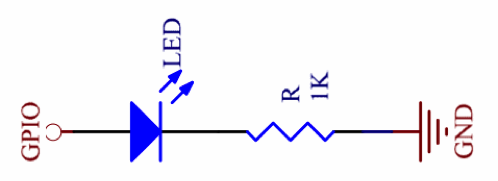
\includegraphics[width=10cm]{figs/ActiveHighLED}}
 \end{center}
                                                            
 
\item [1.2.] Using positive logic (active high) connect a push-button Switch between 3.3V and GPIO23 and, with a 1kOhm resistor in series, to ground and explain what happens on the webIOPI header webpage. Draw a schematic diagram for this circuit. Afterwards stop the  \webIOPi Code application.
%Repeat the exercise with negative logic, explain it and draw a schematic diagram. 
 
 \hfill [1 mark]\\
      

\item [1.3.]  Connect an LED with a 1~kOhm resistor as in checkpoint 1.1 above. Start python interactively to set GPIO 24.   Using the templates, import the webiopi framework, make a GPIO object and turn the LED on and off.
%
\begin{verbatim}
    studentn@dahpimm  ~ $ sudo python3
\end{verbatim}
\lstinputlisting{../scripts/checkpoint_1a.py}


Write the first Python script to blink an LED for either positive or negative logic 
by adding a "while loop".\\

\lstinputlisting{../scripts/checkpoint_1b.py}
\vspace*{-0.5cm}
\hfill [2 marks]\\


\item [1.4.]	  Connect the push button switch using  using negative logic (active low)  and the LED circuit with positive logic (active high).  Write a python script to toggle the LED status every time the push button switch is pushed. \\
%once using negative logic for the push button switch. Connect the push and positive logic for the LED. \\

\lstinputlisting{../scripts/checkpoint_1c.py}
\vspace*{-0.5cm}
\hfill [2 marks]\\


\end{enumerate}



\newpage
\section{Checkpoint 2: ADC, DAC and SPI BUS}

Most experimental observables are continuous: their values can vary by arbitrarily small amounts.
However, we record measurements as discrete values: a number with some range of uncertainty.
Creating a numerical (digital) measurement from a continuous (analogue) signal is called digitisation, and is performed by an Analogue to Digital Converter (ADC).
The digital information can then be manipulated with a computer.

In this checkpoint we will use an ADC to read information from a light sensor into the Raspberry Pi.
We will also perform the opposite task, varying the brightness of an LED by converting a numerical output from the Raspberry Pi into the corresponding voltage level using a Digital to Analogue Converter (DAC).

\vspace*{-0.5cm}
\begin{enumerate}

\item [2.1.] Connect an ADC MCP3208 chip to the Raspberry Pi using the SPI Interface on pin GPIO 8 (SPI\_CE0).
Make sure that all required connections between the MCP3208 and the Raspberry-Pi are made (see pin-out sheet).
Use a multimeter to check that power (VDD) and ground (AGND and DGND) are correctly connected.
Explain what all connections are for.

Connect a Light Dependent Resistor (LDR) and a 4.7~k$\Omega$ resistor as a voltage divider between 3.3 and 0~V, using an ADC input channel to measure the voltage in the middle.
Use python interactively to read the voltages of all eight ADC channels.
Try reading a specific ADC channel, and experiment with all the other methods given below.
You are encouraged to consult the following webpage \url{http://webiopi.trouch.com/}($\rightarrow$ Tutorials $\rightarrow$ Using Devices $\rightarrow$ Analogue).

Explain how the ADC works and what the meaning of the return values of each method is.
What is the primary ADC output and how is the voltage output calculated from this?
Cover the LDR with your hand, and explain how the ADC readings change. \\

\lstinputlisting{../scripts/checkpoint_2a.py}
\vspace*{-0.5cm}
\hfill [3 marks]\\

%\newpage
\item [2.2.] Leave the ADC in place, but also connect the DAC MCP4922 chip to the Raspberry-Pi using the other SPI Interface on GPIO 7 (SPI\_CE1).
Make sure that all required connections between the MCP4922 and the Raspberry-Pi are made (see pin-out sheet).
Use a multimeter to check that power (VDD) and ground (AVSS) are correctly connected.
Explain how the DAC works and what all connections are for.

Use python interactively to set a value --- e.g. 1.3 V --- to output VOUTA of the DAC.
Measure this voltage with a multimeter. \\

\lstinputlisting{../scripts/checkpoint_2b.py}
\vspace*{-0.5cm}
\hfill [2 marks]\\

\item [2.3.] Connect one output of the DAC to an LED.
Write a python script that varies the brightness of the LED by setting a series of different values for the output voltage of the DAC.
Now arrange the circuit so that the LED is next to the LDR, and the change in brightness can be measured.
The laboratory is quite bright relative to an LED, so you might need to cover the breadboard to show a convincing change.
Modify your script to read the ADC input each time you set the DAC output.
Write the DAC setting and measured ADC values at each step to an output file with comments such that the content of the file will explain your work.


\hfill [3 marks]\\

\end{enumerate}



\newpage
\section{Checkpoint 3:  Generating and Sampling Analogue Signals}

\begin{enumerate}

\item [3.1.] Connect an ADC chip (MCP3208) to the Raspberry Pi, as in Checkpoint 2. Verify that the ADC works with a DC voltage produced with a potentiometer.

Use the signal generator to produce a repetitive signal, e.g. a sinusoidal waveform. Display the output on the oscilloscope. Set the amplitude of the signal such that the waveform can be read by the ADC chip, which can sample between 0 V and VREF = 3.3 V. Set the frequency to 10 Hz.  

Connect the output of the signal generator to an ADC input channel. Using python in interactive mode read a few samples of the ADC output. Comment on what you measure. [Caveat: Don't connect a signal with a voltage outside the range of the ADC chip, which could destroy it and the Raspberry Pi.] 

\hfill [1 marks]\\

\item [3.2.] Measure the waveform produced by the signal generator by writing a python script that records 100 ADC samples and displays these on a graph. Always label plots correctly with title and axes and save these to a file (pdf format). 
[Hint: Use the pylab interface for plotting graphs as discussed in the python tutorial. Example files are available on github. ]

\hfill [2 marks] \\

\item [3.3.] Calibrate the voltage scale of the ADC output with respect to the oscilloscope by using a square waveform that matches the ADC input range.  First connect the signal from the signal generator to the oscilloscope and read the input voltage for the high and low sections of the square waveform off the oscilloscope screen. (Use the trigger threshold dial to determine these quite precisely). Then connect the signal to an ADC input channel. Write a python script that takes 100 ADC samples and writes these onto the screen or into a file. Determine the average ADC values for the high and low sections of the square waveform and plot these versus the two input voltages. Reduce the amplitude of the input waveform by a factor of two and repeat above procedure.  Plot the four calibration measurements on a graph and comment.

\hfill [2 marks] \\

\item[3.4.]	What is the maximum signal frequency with which you can properly record a given repetitive signal?  Consider which would be the best waveform for this investigation. What is the sampling frequency? Explain what happens when a signal is undersampled. Make a plot with a waveform that is undersampled.   

\hfill [2 marks] \\

\item [3.5.] Connect a DAC chip (MCP4922) to the Raspberry Pi, as in Checkpoint 2.  Using a python script, generate a sinusoidal waveform on the DAC output and plot the waveform to a graph.

Use the ADC chip (MCP3208) to digitise the waveform generated by the DAC. Write a python script that takes 100 DAC samples and 100 ADC measurements and plot these on the same graph. Take into account the limitations encountered in 3.4.                                                          
 
\hfill [3 marks] 

\end{enumerate}


\newpage
\section{Checkpoint 4: Input/Output I/O and I2C BUS}

\begin{enumerate}


\item [4.1.] Input/Output (I/O) Expander chips enable the user to connect many devices having the same or similar functions.  With the Raspberry Pi this can be achieved using the I2C bus. Connect the PCF8574AN chip  (I2C BUS Expander) to the Raspberry-Pi. Make sure that all required connections between the PCF8574AN chip and the Raspberry-Pi are made, see pin-out sheet. Explain how the I/O Expander works and what the SDA, SCL and A0, A1, A2 address lines are. 
%\hfill [2 marks]\\

%\item [4.2.] 
Using negative logic connect an LED to output P0 of the PCF8574AN Expander chip. 
Write a python script to blink the LED using negative logic, see checkpoint 1 for setting up a while loop.  Why is negative logic necessary? 

You may consult the \webiopi webpage  \url{http://webiopi.trouch.com/} ($\rightarrow$ Tutorials $\rightarrow$ Using Devices $\rightarrow$ Digital) to find information on the GPIO expander chip. \\

\lstinputlisting{../scripts/checkpoint_4a.py}
\hfill [3 marks]\\

\item [4.2.] Connect an additional 3 LEDs to outputs P1, P2 and P3 of the PCF8574AN Expander chip. Write a python script which turns the LEDs on and off in a predefined pattern, such as a running light. Consider P0 to P3 as default, but you are encouraged to play with other patterns. 

\hfill [2 marks]\\

\newpage
\item [4.3.] Consult the webpage \url{http://webiopi.trouch.com/} ($\rightarrow$ Tutorials $\rightarrow$ Using Devices $\rightarrow$ Digital) for the GPIO Expander. Use the portWrite(value) method to manipulate all four LEDs at the same time.  Connect a push button switch to pin P4 of the expander chip. Write a python script such that an LED pattern toggles every time the button is pushed.\\

\lstinputlisting{../scripts/checkpoint_4b.py}
\hfill [3 marks]\\


\end{enumerate}



\newpage
\section{Checkpoint 5: Temperature Sensors}

\begin{enumerate}

\item [5.1.] We will be using DS18B20 temperature sensors for this checkpoint. Take a look at the datasheet here: http://www.adafruit.com/datasheets/DS18B20.pdf  or download it from the DAH Dropbox.

Connect a DS182B0 temperature sensor to your Raspberry pi (look at the flat front of the sensor to get it the right way around):
\begin{center}
    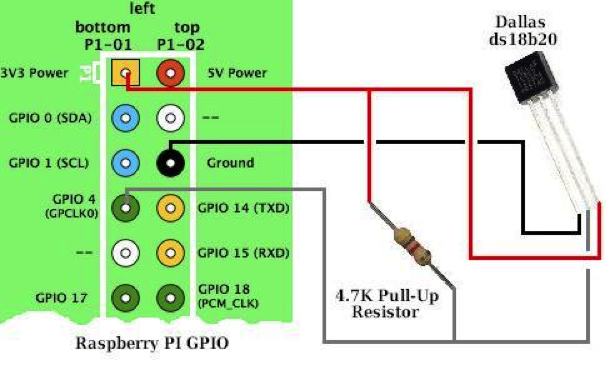
\includegraphics[width=14cm]{figs/DS182B0}
\end{center}

What is the interface between the DS18B20 temperature sensor and the Raspberry Pi? Explain how it works. 

\begin{comment}
Install the drivers for the sensor on the Raspberry Pi with the following commands:
    pi@Demonstrator-pi ~ $   sudo modprobe w1-gpio
    pi@Demonstrator-pi ~ $   sudo modprobe w1-therm

Note that you will need to do this again if you restart the Raspberry Pi.
\end{comment}

Locate the sensor output by finding the file that has the serial number of your sensor:
\begin{verbatim} 
    studentn@dahpimm ~ $  cd /sys/bus/w1/devices 
    studentn@dahpimm /sys/bus/w1/devices $ ls 
    10-00080265b6d6 w1_bus_master1 
\end{verbatim}
where n = 1 to 50 and mm = 01 to 22.
Note that your temperature sensor won't be called 10-00080265b6d6, this is just an example.

Now read the sensor output, i.e. the raw temperature measurement:
\begin{verbatim}
    studentn@dahpimm /sys/bus/w1/devices ~ $ cd 10-00080265b6d6
    studentn@dahpimm /sys/bus/w1/devices/10-00080265b6d6 $ cat w1_slave 
    30 00 4b 46 ff ff 0d 10 29 : crc=29 YES 
    30 00 4b 46 ff ff 0d 10 29 t=23937 
\end{verbatim}
    
This should be interpreted as 23.937 centigrade (degree Celsius). 

\newpage
WebIOPi provides a simple way to access the temperature sensor data in python. It is best to test this by running python in interactive mode first.  
\begin{verbatim}
    studentn@dahpimm ~ $ python3
\end{verbatim}
\lstinputlisting{../scripts/checkpoint_5a.py}
\hfill [2 marks]


\item[5.2.] Measure temperature with the DS18B20 sensor versus time. Choose a sensible time interval. Write a python script to make a graph of 50 temperature measurements versus time. Always label plots correctly with title and axes and save these to a file.
 
As a second step the graph should update itself as each temperature measurement is made. Write a python script for this purpose.  Once this is working, play with it by touching the temperature sensor with you fingers. Describe what is happening and sketch it in your lab book.

The following code example shows how to display a plot that updates regularly:\\

\lstinputlisting{../scripts/checkpoint_5b.py}
\hfill [3 marks]



\item[5.3.]	Add another temperature sensor to your circuit by connecting it in parallel with the existing one. You don't need to make separate connections to the Raspberry Pi: your new sensor can share these with the existing one (Just make sure that you connect it the right way around).

Find its serial number in the w1/devices folder like before. Now ensure that you can read out your two temperature sensors simultaneously in python. You can test this by running python in interactive mode first. 
Note that your temperature sensors will have different serial numbers.

\begin{verbatim}
    studentn@dahpimm  ~ $ python3
\end{verbatim}
\lstinputlisting{../scripts/checkpoint_5c.py}

What is the smallest change in temperature that a sensor can report? Explain this with reference to the datasheet, and how the temperature information is encoded.

Investigate the accuracy of the sensor readings by looking at the stability of the measurement with time, and by comparing the outputs of your two sensors. You can probably assume that the ambient temperature in the lab is constant, but shielding your sensors from breezes may help.

Modify your graphing code from part 5.2 to make histograms of the temperature measurements of the two sensors. 

You can use the pylab histogram command:\\
\lstinputlisting{../scripts/checkpoint_5d.py}
Make also a graph of the difference between the temperature of the two sensors. Determine the RMS value of a set of temperature difference measurements between the two sensors. Explain your results. Are these consistent with the datasheet?

\hfill [3 marks]


\end{enumerate}


\newpage
\section{Checkpoint 6: Data Handling and Analysis}

\begin{enumerate}

\item [6.1.] This is a data handling exercise and the Raspberry Pi is not required.
Thus this checkpoint is best carried out using the Physics CPlab computers. 
There is a CPlab computer available on every desk in the DAH laboratory.
You can use the following python libraries. \\

\lstinputlisting{../scripts/checkpoint_6a.py}

The LHCb experiment at the Large Hadron Collider at CERN has recorded a sample of muon pairs with invariant masses in the range of 8.5 to 11 GeV/$c^2$. Three clear peaks are observed in this mass spectrum. These correspond to the production of Upsilon mesons, which are bound states of a $b$ and a anti-$b$ quark. These states are known as the $\Upsilon \rm (1S)$, $\Upsilon \rm (2S)$ and $\Upsilon \rm (3S)$ mesons where the $\Upsilon \rm (1S)$ meson is the ground state and the $\Upsilon \rm (2S)$  and $\Upsilon \rm (3S)$  states are radial excitations (for LHCb paper, see {DOI: 10.1007/JHEP06(2013)064).}

\begin{center}
    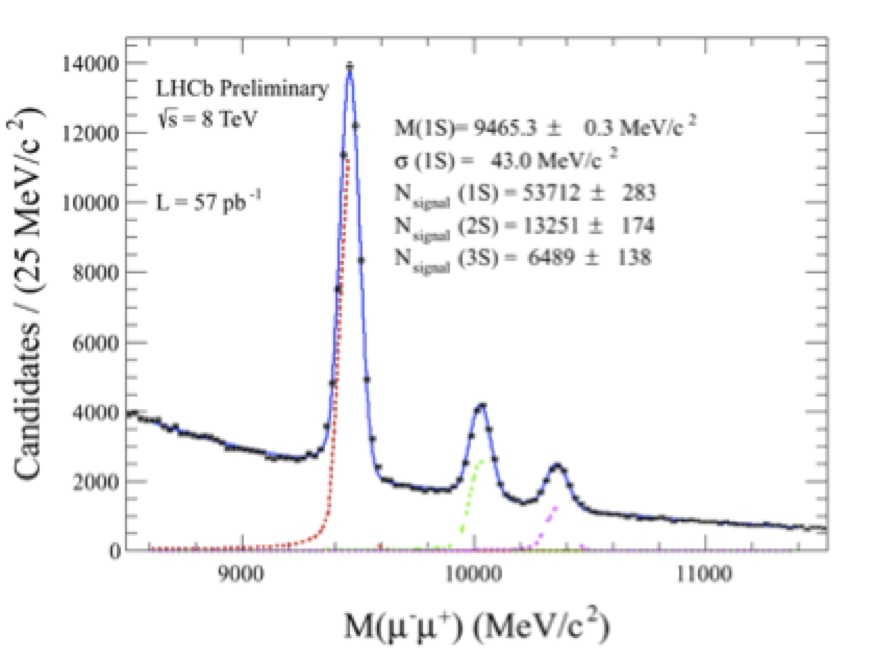
\includegraphics[width=9cm]{figs/mu-pair-mass}
\end{center}

Download the file upsilons-mass-xaa.txt from the DAH Dropbox, which contains the invariant masses of a large number of muon pairs in units of GeV/$c^2$ in text format. Write a python script that reads the data from this file and plots a histogram of all the masses, choosing a reasonable bin width. Always label plots correctly with title and axes and save these to a file.
[Hint: The bin width should be chosen such that each of the three peaks is clearly resolved and represented by a sufficient number of bins for analysis.]

\hfill [2 marks]


\item [6.2.] Determine the masses of the three particles by determining the bins with the highest number of entries in the peak regions. Divide the histogram into three peak regions and write a local peak finding method for this part.
What are the mass differences between the $\Upsilon \rm (2S)$ and $\Upsilon \rm (3S)$ states with respect to the $\Upsilon \rm (1S)$ meson? By inspecting visually the muon-pair mass
spectrum, determine the Full Width Half Maximum (FWHM) of the $\Upsilon \rm (1S)$ mass peak.

\hfill [2 marks]


\item [6.3.] Determine the mass of the  $\Upsilon \rm (1S)$  meson and its statistical uncertainty. This can be achieved by several methods. First by looking at the mass spectrum, choose a suitable region around the $\Upsilon \rm (1S)$  mass peak. Calculate the mean, the unbiased variance and standard deviation for the events in this region. Use these values to determine the standard deviation of the mean. Comment on possible biases for this method. 


The mass peaks corresponding to the three $\Upsilon$ mesons can be described 
reasonably well by a Gaussian function, 
$f(x) = \frac{N}{\sigma \sqrt{2\pi}}  \exp{\left( - \frac{(x-/\mu)^2}{2\sigma^2} \right)} $
where $x$ is the invariant mass of the muon pairs, $\mu$ is the mass of the $\Upsilon \rm (1S)$  meson, $\sigma$ is the Gaussian width (mass resolution) and $N$ is the total number of signal events. 
Estimate the mass resolution $\sigma$ from the FWHM of the $\Upsilon \rm (1S)$  peak. Compare the mass resolution with the standard deviation in the signal region determined above.

\hfill [2 marks]\\


In the muon-pair mass spectrum define a signal region of width $\pm 150\; {\rm MeV}/c^2$ around the $\Upsilon \rm (1S)$  peak position and determine the number of events $N$ in this region. 
Define an upper and lower sideband region where there are only background events. These sidebands should each be half as wide as the signal region and located at masses equidistant from the $\Upsilon \rm (1S)$  peak position. Assuming that the background is falling linearly with the muon-pair mass, determine the number of background events $B$ in the signal region (below the $\Upsilon \rm (1S)$  mass peak). Perform either a linear least squares fit in the sideband regions or use the sideband subtraction method for this. Determine the number of signal events $S$ in the signal region.

Alternatively, if you know how to perform a fit you may choose fitting the $\Upsilon \rm (1S)$   peak in the mass spectrum for this part.

% Assuming Gaussian statistics for N and using the mass resolution ? determine the statistical error %on the mass of the ?(1S) meson. 
Compare your mass measurement with the Particle Data Group (\url{pdg.lbl.gov}) and comment.
[Hint: The PDG lists the properties of particles. Select "pdgLive - Interactive Listings" followed by "Mesons b anti-b" to find the $\Upsilon \rm (1S)$  meson.]

\hfill [3 marks]

\begin{comment}

6.4. Download the file upsilons-mass-pt-xaa.txt from the DAH Dropbox which, in addition to the masses, also contains the transverse momenta pT of the muon- pairs in units of GeV/c in text format. For an explanation of the transverse momentum, see the LHCb paper, referred to above. Write a python script that reads in these data and plot a histogram of the transverse momenta for all events. Plot a 2-dimensional histogram of pT versus mass for all events, choosing 50 bins in pT and 100 bins in mass.
[Hint (python):]
%# Splitting a line with two strings separated by a blank space line = line.split()
12
[1 mark]

\end{comment}



\end{enumerate}


\chapter{DAH Projects}
\label{sec:projects}
%
All the projects involve analysis of data taken by the LHCb experiment. For more information on LHCb you are refered to  {DOI:10.1007/JHEP06(2013)064).}. The data is presented to allow you to do this in a simplified way but the steps you will follow are similar to what is done in any real analysis
\begin{itemize}
\item Make simple checks of the data, for example making histograms and using these to estimate the position and width of peaks.
\item Perform fits to invariant mass distributions to determine the yield of particles.
\item Apply cuts to improve the signal to background or to select a specific region of space space.
\item Compare your results to theory expectations and previous studies.
\end{itemize}
The projects have been designed in to explore the data in different ways and to chose your own adventure. They all start from binary files which store around six different variables for different datasets collected by LHCb. The meaning of these variables may not be immediately clear to you at the start of the project and this is something you will need to think about. You should think  about what the advantages and disadvantages of storing binary information are. Some of the data files used in the project are rather large. Fitting large datasets without binning can be computationally challenging and you may consider a binned fit if appropriate.

We are assuming for the projects that all of you have a laptop and will on this remotely. If you need access to the CPLab computers on the desks in the DAH laboratories to perform the project you should contact the course organizers.

\section{Project F1: Make Accurate Measurements of $\Upsilon$  Masses}

\subsection{Goals of project}
%
You will use LHCb data on the invariant mass of $\Upsilon$ particle candidates collected in 2015. You will first make simple checks of the data and get first estimates of peak positions and widths.  Next you will use the maximum likelihood process to fit different mass model shapes to the data. From this you will determine the parameters of the mass model for the three signal peaks, and their errors. You will start with a very simple Gaussian mass model. You will then improve this and use a more sophisticated model.

The project has an open-ended aspect and are an opportunity where you can show your own initiative and demonstrate your experimental and computational skills. 

\subsection{Detailed project description}

The LHCb experiment at the Large Hadron Collider at CERN has recorded a sample of muon pairs with invariant masses in the range of 8.5 to 11 GeV/$c^2$. Three clear peaks are observed in this mass spectrum. These correspond to the production of Upsilon mesons, which are bound states of a $b$ and a anti-$b$ quark. These states are known as the $\Upsilon \rm (1S)$, $\Upsilon \rm (2S)$ and $\Upsilon \rm (3S)$ mesons where the $\Upsilon \rm (1S)$ meson is the ground state and the $\Upsilon \rm (2S)$  and $\Upsilon \rm (3S)$  states are radial excitations (for LHCb paper, see {DOI: 10.1007/JHEP06(2013)064).}

\begin{center}
    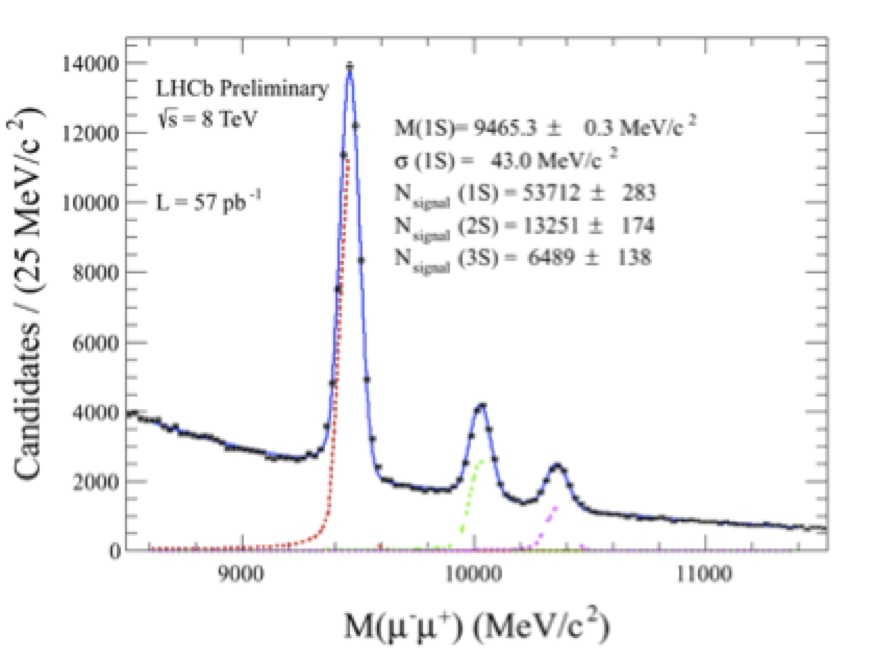
\includegraphics[width=9cm]{figs/mu-pair-mass}
\end{center}

Download the files ups-15.bin, ups-15-small.bin and mc.bin   from the DAH Dropbox, 
The first  two files contain the data recorded by LHCb in 2015 and a subset with a factor 5 less data. 
In addition, there is a file with simulated data (Monte Carlo).
The files are written in binary format and contain five observables for a large number of muon pairs
\begin{itemize}
\item  invariant mass of muon pair in   GeV/$c^2$;
\item transverse momentum $p_\perp$ of muon pair in GeV/$c$;
\item rapidity $\eta$ of muon pair;
\item  momentum $p$ of muon pair in GeV/$c$;
\item transverse momentum $pt$ of first muon in GeV/$c$;
\item transverse momentum $pt$ of second muon in GeV/$c$.
\end{itemize}

Write a python script that reads the data from this file, see below. 

\lstinputlisting{../scripts/project_F_a.py}
\vspace*{-0.5cm}

Start with the small ups-15-small.bin file. Plot histograms of all six variables, choosing a reasonable bin width. Always label plots correctly with title and axes and save these to a file. [Hint: The bin width should be chosen such that each of the three peaks is clearly resolved and represented by a sufficient number of bins for analysis.]

Next, make some estimates of the peak positions and widths using the histogram of invariant mass.  Determine the masses of the three particles by determining the bins with the highest number of entries in the peak regions. Divide the histogram into three peak regions and write a local peak finding method for this part.
What are the mass differences between the $\Upsilon \rm (2S)$ and $\Upsilon \rm (3S)$ states with respect to the $\Upsilon \rm (1S)$ meson. By inspecting visually the muon-pair mass spectrum, determine the Full Width Half Maximum (FWHM) of the $\Upsilon \rm (1S)$ mass peak. Assuming a Gaussian signal shape estimate the mass resolution $\sigma$ from the FWHM. %of the $\Upsilon \rm (1S)$  peak.

In the muon-pair mass spectrum define a signal region of width $\pm 150\; {\rm MeV}/c^2$ around the $\Upsilon \rm (1S)$  peak position and determine the number of events $N$ in this region.
Define an upper and lower sideband region where there are only background events. These sidebands should each be half as wide as the signal region and located at masses equidistant from the $\Upsilon \rm (1S)$  peak position. Assuming that the background is falling linearly with the muon-pair mass, determine the number of background events $B$ in the signal region (below the $\Upsilon \rm (1S)$  mass peak). Perform either a linear least squares fit in the sideband regions or use the sideband subtraction method for this. Determine the number of signal events $S$ in the signal region.

\begin{enumerate}
\item Consider first the $\Upsilon \rm (1S)$ particle, which is the particle with the lowest mass, i.e. the left most  peak in the plot. Construct a composite probability density function (PDF) for the invariant mass of the muon pairs, which contains two components:
\begin{itemize}
\item A Gaussian shape to fit the  $\Upsilon \rm (1S)$ mass peak;
\item A shallow falling exponential to fit the background shape of the mass spectrum underneath and around the peak.
\end{itemize}

\item Use this PDF in a Maximum Likelihood fit to determine the parameters of the PDF. Note that it is essential that the composite PDF remains normalised to 1 over the range of the fit.

Determine the $\Upsilon \rm (1S)$  meson mass and yield, and all other parameters, and their and errors.

You should be able to obtain the parameter errors directly from the minimization engine of your choice (scipy.optimize.minimise, scipy.optimise.curve\_fit, lmfit, see \url{https://lmfit.github.io/lmfit-py/} or Minuit). Depending on your choice you will be able to chose different minimising methods.
It would be good to show that you understand these by obtaining them yourself from the parameters of the Gaussian signal fit - this is described in the data handling lectures.

Plot the fitted signal shape on top of the data.

\item Now consider the entire mass range, and perform a simultaneous fit for all three Upsilon peaks, and the underlying background. Again you should always report the parameter values, and their errors. Plot the fitted signal shape on top of the data.

\item The results so far probably look "quite good" by eye.  i.e. the signal shape plotted on top of the data probably looks like it fits quite well.  However this can be misleading when performing a precision measurement.  You should make a plot of what are called the "residuals". A residual is the difference between the data in the binned histogram and the best-fit mass model value for the centre of that bin. Describe what you see.

\item There are several ways to enhance the scope of the project. For example, if the single Gaussian mass model does not fit the data perfectly, one can try other mass models, i.e. by using a signal PDF that goes beyond a single Gaussian function.  Examples are:
\begin{itemize}
\item A PDF comprising a function which is the sum of two Gaussian functions (i.e. one narrow and one wide Gaussian function to fit a single Upsilon mass peak)
\item A Crystal Ball function, which incorporates a non-Gaussian tail at the lower end of the mass peak. The functional shape is described elsewhere, e.g. see: \url{http://en.wikipedia.org/wiki/Crystal_Ball_function}. 
\end{itemize}
Implement one or both of these functions in your PDF. 
First fit this PDF using the simulated Monte Carlo data. This allows you to see better
how the additional parameters should improve the description of the tails of the signal peak.
Then fit the PDF to the LHCb data and see how much better they are at describing the data.
Consider fixing some of the shape parameters from the fit to the Monte Carlo sample.

\item Make 2-dimensional plots of the additional observables vs the invariant mass of the muon pair.
Find out if you can improve the purity of your signal sample using the information in the file.
The purity is defined as the ratio of signal events over all events in a region.

\item As on open ended activity, you will see in the paper that the analysis is also done by dividing the data up into bins of transverse momentum ($pt$) and pseudorapidity ($\eta$). You can explore doing this analysis yourself and try to make the cross-section in bins of pT or eta. In particular taking ratios of yields will allow you to cancel the detector acceptance.
  
\item Read the publication and see what is said about systematic errors.  Make a reasonable attempt at determining some systematic errors on the masses.


\end{enumerate}

\subsection{Project planning}

The project descriptions are generally significantly less detailed than what was made available for the checkpoints. Any material covered during checkpoints including python code examples are assumed to be known.  Only essential and new information is provided and you are expected to take care of the details. Python code snippets are provided where necessary, but you will have to understand yourself what they do. It is recommend that you google for information about your project on the web, including data sheets of components and python libraries, if applicable. Python scripts should be well structured, either using functions or classes.

The timeline will vary between different projects, but in general, it is recommended that you plan your work as follows:
\begin{itemize}
\item	weeks 7, 8 \& 9: 	Building your gadget and/or writing code for project;
\item	week 9, 10: 	Analysis of data or equivalent, prepare supplementary material;
\item	week 10, 11:	Finish writing of project report and prepare submission.
\end{itemize}
Note that you are advised to start writing your report as the project progresses. 

For guidance on report writing, how the projects will be assessed, plagiarism and the submission deadline, please consult the DAH course booklet and the DAH grade descriptors, available on Learn.

 
 
 
\newpage
\section{Project F2: Make Accurate Measurements of Open charm meson Masses}
%
You will use LHCb data to study the mass of open charm mesons. You will first make simple checks of the data and get first estimates of peak positions and widths. You will use the maximum likelihood process to fit different mass model shapes to the data. From this you will determine the parameters of the mass model for the signal peaks, and their errors. You will start with a very simple Gaussian mass model. You will then improve this and use a more sophisticated model. 

The projects have an open-ended aspect and are an opportunity where you can show your own initiative and demonstrate your experimental and computational skills.



\subsection{Detailed project description}
 
In this project you will explore another LHCb dataset collected in 2011 where a pair of
oppositely charged kaons and a pion have been combined. Two clear
peaks are observed in this mass spectrum corresponding to the $D_s^+$ (quark content $c\overline{s}$)
and $D^+$ (quark content $c\overline{d}$) mesons (charge conjugation is implied), see figure below % (Fig.~\ref{fig:dmass}). 
For more information see: {DOI:10.1007/JHEP06(2013)065}. 
%
%\begin{figure}[htb!]
\begin{center}
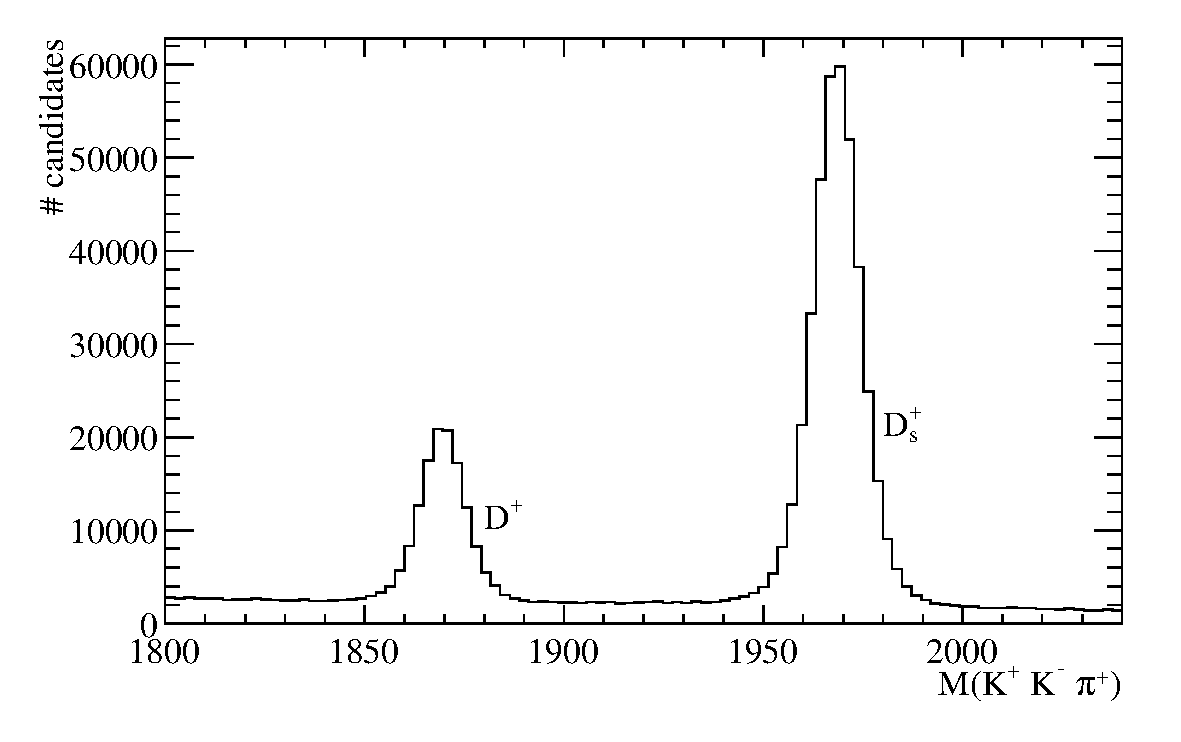
\includegraphics[width=0.75\textwidth]{figs/KKpi.pdf}\\
%\caption
{\small $K^{+}K^{-}\pi^{+}$ invariant mass distribution.}
%\label{fig:dmass}
\end{center}
%\end{figure}
%

Download the files kkp.bin and kkpp.bin files  from the DAH Dropbox, 
These files contain the data recorded by LHCb in 2011 for $D_{(s)}^+$ and $D^0$ decays respectively. Focus on the $D_{(s)}^+$ data file (kkp.bin):
The files are written in binary format and contain seven observables
\begin{itemize}
\item  invariant mass of $K^{+}K^{-}\pi^{+}$  candidate  in  MeV/$c^2$;
\item  invariant mass of kaon pair in   MeV/$c^2$;
\item transverse momentum of  $K^{+}K^{-}\pi^{+}$  candidate  in GeV/$c$;
\item rapidity $\eta$ of $K^{+}K^{-}\pi^{+}$  candidate;
\item minimum tranverse momentum of the three tracks in the $K^{+}K^{-}\pi^{+}$  candidate;
\item electric charge of the candidate;
\item Polarity of the LHCb magnetic field.
\end{itemize}

Write a python script that reads the data from this file, see below. 
\lstinputlisting{../scripts/project_F_b.py}
%\vspace*{-0.5cm}

\begin{enumerate}

\item Plot histograms of all variables, choosing a reasonable bin width. Always label plots correctly with title and axes and save these to a file. [Hint: The bin width should be chosen such that each of the three peaks is clearly resolved and represented by a sufficient number of bins for analysis.]

\item Next, make some estimates of the peak positions and widths using the histogram of invariant mass.  Determine the masses of the two particles by determining the bins with the highest number of entries in the peak regions. Divide the histogram into two peak regions and write a local peak finding method for this part. What is the mass differences between the $D_s^+$ and $D^+$ state ? By inspecting visually the mass spectrum, determine the Full Width Half Maximum (FWHM) of the $D_s^+$ mass peak. Assuming a Gaussian signal shape estimate the mass resolution $\sigma$ from the FWHM.

\item In the  $K^{+}K^{-}\pi^{+}$  mass spectrum define a signal region of width $\pm 25\; {\rm MeV}/c^2$ around the $D_s^+$  peak position and determine the number of events $N$ in this region.
Define an upper and lower sideband region where there are only background events. These sidebands should each be half as wide as the signal region and located at masses equidistant from the $D_s^+$  peak position. Assuming that the background is falling linearly with the mass, determine the number of background events $B$ in the signal region (below the $D_s^+$ peak). Perform either a linear least squares fit in the sideband regions or use the sideband subtraction method for this. Determine the number of signal events $S$ in the signal region.

\item Consider first the $D_s^+$ peak which is the particle with the higher
mass, i.e. the right most peak in the plot. Construct a composite probability density
function (PDF) for the invariant mass of the muon pairs, which
contains two components : 
\begin{itemize}
\item A Gaussian shape to fit the  $D_s^+$ mass peak;
\item A shallow falling exponential to fit the background shape of the mass spectrum underneath and around the peak.
\end{itemize}

\item	Use this PDF in a Maximum Likelihood fit to determine the parameters of the PDF. Note hat it is essential that the composite PDF remains normalised to 1 over the range of the fit.

Determine the $D^+$  meson mass and yield, and all other parameters, and their and errors.

You should be able to obtain the parameter errors directly from the minimization engine of your choice (scipy.optimize.minimise, scipy.optimise.curve\_fit, lmfit, see \url{https://lmfit.github.io/lmfit-py/} or Minuit). Depending on your choice you will be able to chose different minimising methods.
It would be good to show that you understand these by obtaining them yourself from the parameters of the Gaussian signal fit - this is described in the data handling lectures.

Plot the fitted signal shape on top of the data.

\item Now consider the entire mass range, and perform a simultaneous fit for both
peaks, and the underlying background. Again you should always report the parameter
values, and their errors. Plot the fitted signal shape on top of the data.
\item The results so far probably look quite good by eye. i.e. the signal shape plotted on
top of the data probably looks like it fits quite well. However this can be misleading
when performing a precision measurement. You should make a plot of what are called
the residuals. A residual is the difference between the data in the binned histogram
and the best-fit mass model value for the centre of that bin. Describe what you see.
\item There are several ways to enhance the scope of the project.

\begin{itemize} 
\item For example, if the single
Gaussian mass model does not fit the data perfectly, one can try other mass models,
i.e. by using a signal PDF that goes beyond a single Gaussian
function. One example: is a PDF comprising a function which is the sum of two Gaussian functions (i.e. one
narrow and one wide Gaussian function to fit a single $D_{(s)}$ meson
peak. Alternatively try a Crystal Ball function, which incorporates a non-Gaussian tail at the lower end of
the mass peak. The functional shape is described elsewhere, e.g. see:
\begin{verbatim}
https://en.wikipedia.org/wiki/Crystal_Ball_function 
\end{verbatim} 
You could implement each of these functions in your PDF and see how much better
they are at describing the data.
\item Read the publication and see what is said about systematic errors. Make a reasonable
attempt at determining some systematic errors on the masses.
\item Compare your results to the PDG and previous measurements.
\item Study how the mass and the width of the peak (the resolution)
  depends on the transverse momentum (pt) and rapidity (eta).
\item In the data file you are provided with the charge of the D meson and the magnetic field polarity. Divide up the data into different categories of charge and polarity and remake the fits. What can you learn from these studies ?
\item Investigate whethe the mass of kaon pair and the minimum tranverse momentum of the
 daughter particles can be used to improve the purity of the sample.
\item An additional file has been provided of candidates for the decay $D^0 \rightarrow K^+ K^- \pi^+ \pi^-$. Use this file to estimate the mass splitting between the charged and neutral D mesons and compare to the PDG. The variables in this file are the candidate mass, the mass of the kaon pair, pt, eta, ptmin and field polarity.
\end{itemize}



\end{enumerate}

\subsection{Project planning}

The project descriptions are generally significantly less detailed than what was made available for the checkpoints. Any material covered during checkpoints including python code examples are assumed to be known.  Only essential and new information is provided and you are expected to take care of the details. Python code snippets are provided where necessary, but you will have to understand yourself what they do. It is recommend that you google for information about your project on the web, including data sheets of components and python libraries, if applicable. Python scripts should be well structured, either using functions or classes.

The timeline will vary between different projects, but in general, it is recommended that you plan your work as follows:
\begin{itemize}
\item	weeks 7, 8 \& 9: 	Building your gadget and/or writing code for project;
\item	week 9, 10: 	Analysis of data or equivalent, prepare supplementary material;
\item	week 10, 11:	Finish writing of project report and prepare submission.
\end{itemize}
Note that you are advised to start writing your report as the project progresses. 

For guidance on report writing, how the projects will be assessed, plagiarism and the submission deadline, please consult the DAH course booklet and the DAH grade descriptors, available on Learn.

 

\newpage
\section{Project F3: Production of $J/\psi$ mesons}

\subsection{Goals of project}

You will use LHCb data on the the production and properties of $J/\psi$ mesons. You will first make simple checks of the data and get first estimates of peak positions and widths. You will use the maximum likelihood process to fit different mass model shapes to the data. From this you will determine the parameters of the mass model for the signal peak, and their errors. You will start with a very simple Gaussian mass model. You will then improve this and use a more sophisticated model.

The project has an open-ended aspect and are an opportunity where you can show your own initiative and demonstrate your experimental and computational skills. 




\subsection{Detailed project description}
 
In this project you will explore an LHCb dataset where the decay a pair of oppositely charged muons originating from the decay of a $J/\psi$ meson ( a $c\overline{c}$ state) is reconstructed. The $J/\psi$ can be produced in different procsses but in this case selection requirements have been applied that select $J/\psi$ produced in decays of the $b$-quark. For more information see  {DOI:10.1007/JHEP1Dro(2015)172}. The data you are using comes from later LHCb running during 2016. A downscale of 10 has been applied but the dataset is still large. 

%
%\Begin{figure}[htb!]
\begin{center}
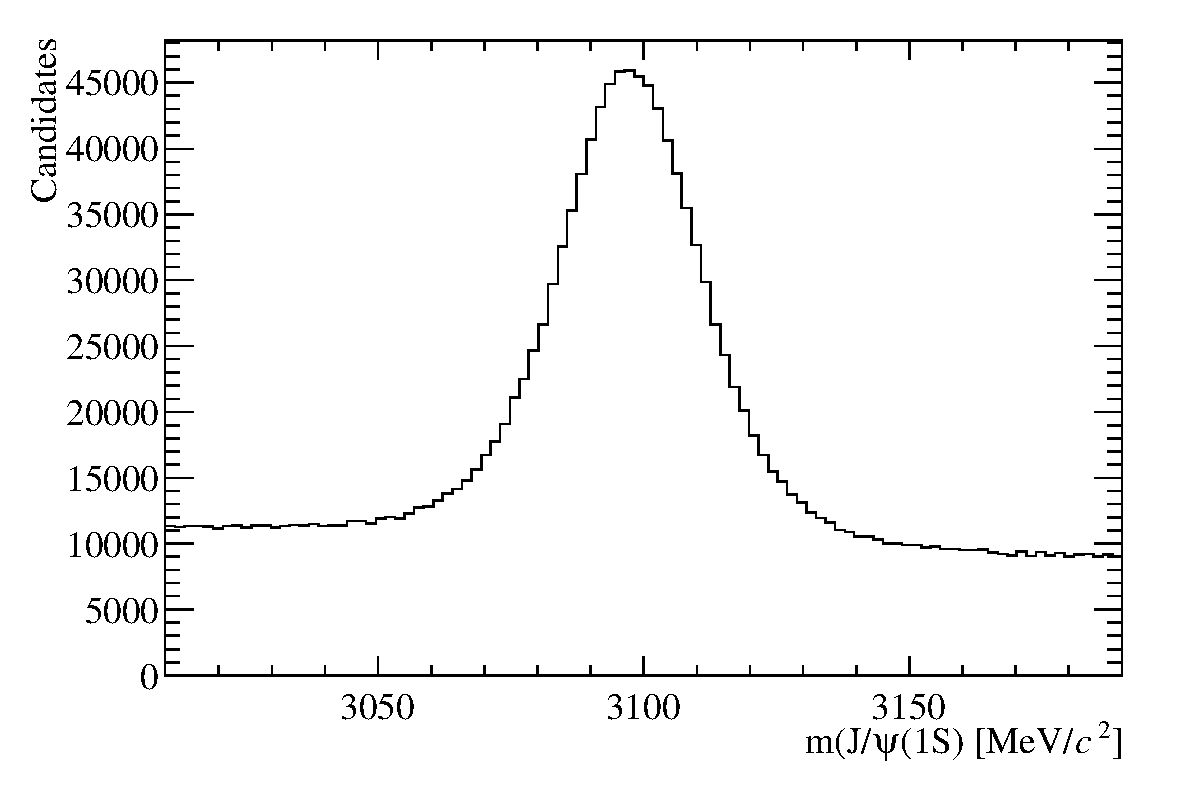
\includegraphics[width=0.75\textwidth]{figs/jpsi.pdf}\\
%\caption
{\small $\mu^+ \mu^-$ invariant mass distribution.}
%\label{fig:dmass}
\end{center}
%\end{figure}
%

Download the files jpsi.bin and jpsi-small.bin files  from the DAH Dropbox. These files contain the data recorded by LHCb in 2016 for $J/\psi \rightarrow \mu^+ \mu^-$ decays respectively. First, focus on the smalld data file (jpsi-small.bin), this contains a subset of the data. The files are written in binary format and contain seven observables for a large number of muon pairs
\begin{itemize}
\item  invariant mass of $J\psi$  candidate  in  MeV/$c^2$;
\item transverse momentum of  the dimuon candidate  candidate in MeV/$c$;
\item rapidity $\eta$ of the dimuon candidate;
\item $\chi^2$ of the geometric vertex of the dimuon candidate; 
\item Minimum transverse momentum of the two muons in MeV/$c$;
\item Minimum of a variable (ProbNNmu) that characterizes how well the two tracks forming the candidate match the hypothesis of being muons;
\item Minimum impact parameter $\chi^2$ of the two muons. The impact parameter characterizes how well the particle is matched as coming directly from a proton-proton interaction. For tracks from
 $b-$decays it should be large.
\end{itemize}

Write a python script that reads the data from this file, see below. 
\lstinputlisting{../scripts/project_F_c.py}
%\vspace*{-0.5cm}

\begin{enumerate}

\item Plot histograms of all seven variables, choosing a reasonable bin width. Always label plots correctly with title and axes and save these to a file. [Hint: The bin width should be chosen such that each of the three peaks is clearly resolved and represented by a sufficient number of bins for analysis.]

\item Next, make estimates of the peak position and width using the histogram of invariant mass.  Determine the mass from the bins with the highest number of entries in the peak regions by writing a local peak finder. By inspecting visually the muon-pair mass spectrum, determine the Full Width Half Maximum (FWHM) of the $J/\psi$ mass peak. Assuming a Gaussian signal shape estimate the mass resolution $\sigma$ from the FWHM.

\item In the  $\mu^{+}\mu^{-}$  mass spectrum define a signal region of width $\pm 30\; {\rm MeV}/c^2$ around the $J/\psi$  peak position and determine the number of events $N$ in this region. Define an upper and lower sideband region where there are only background events. These sidebands should each be half as wide as the signal region and located at masses equidistant from the $J/\psi$  peak position. Assuming that the background is falling linearly with the muon-pair mass, determine the number of background events $B$ in the signal region. Perform either a linear least squares fit in the sideband regions or use the sideband subtraction method for this. Determine the number of signal events $S$ in the signal region.

\item Construct a composite probability density
function (PDF) for the invariant mass of the muon pairs, which
contains two components : 
\begin{itemize}
\item A Gaussian shape to fit the  $J/\psi$ mass peak;
\item A shallow falling exponential to fit the background shape of the mass spectrum underneath and around the peak.
\end{itemize}

\item Use this PDF in a Maximum Likelihood fit to determine the parameters of the PDF. Note that it is essential that the composite PDF remains normalised to 1 over the range of the fit.

Determine the $J/\psi$  meson mass and yield, and all other parameters, and their and errors. Compare the measured mass with was it expected from the PDG.

You should be able to obtain the parameter errors directly from the minimization engine of your choice (scipy.optimize.minimise, scipy.optimise.curve\_fit, lmfit, see \url{https://lmfit.github.io/lmfit-py/} or Minuit). Depending on your choice you will be able to chose different minimising methods.
It would be good to show that you understand these by obtaining them yourself from the parameters of the Gaussian signal fit - this is described in the data handling lectures. Plot the fitted signal shape on top of the data. How does the fitted value of the mass compare to expectations ? 

\item The results so far probably look quite good by eye. i.e. the signal shape plotted on
top of the data probably looks like it fits quite well. However this can be misleading
when performing a precision measurement. You should make a plot of what are called
the residuals. A residual is the difference between the data in the binned histogram
and the best-fit mass model value for the centre of that bin. Describe what you see. Try repeating the exercise using the larger sample.

\item Select only events with an impact parameter $\chi^2$ larger than four and fit the data. Comment on how signal yield and the purity - ie the signal-to-background ratio change.

\item There are several ways to enhance the scope of the project. You may want to use the larger file for some of these studies.

\begin{itemize} 
\item For example, if the single
Gaussian mass model does not fit the data perfectly, one can try other mass models,
i.e. by using a signal PDF that goes beyond a single Gaussian
function. One example: is a PDF comprising a function which is the sum of two Gaussian functions (i.e. one
narrow and one wide Gaussian function to fit a single $J/\psi$ meson
peak. Alternatively try a Crystal Ball function, which incorporates a non-Gaussian tail at the lower end of
the mass peak. The functional shape is described elsewhere, e.g. see:
\begin{verbatim}
https://en.wikipedia.org/wiki/Crystal_Ball_function 
\end{verbatim} 
You could implement each of these functions in your PDF and see how much better
they are at describing the data.
\item Study how the mass and the width of the peak (the resolution)
  depends on the transverse momentum (pt) and rapidity (eta). Think about how the trends you see originate.
\item The fitted yield in bins of  pt and rapidity eta can be compared to the results for $J/\psi$ from b in the paper and with theorectical predictions. For the latter there is an online calculator that can provide you with predictions:
  \begin{verbatim}
  http://www.lpthe.jussieu.fr/~cacciari/fonll/fonllform.html
\end{verbatim} 
\item Investigate if the purity of the sample can be improved by cutting on the other variables in the file.
\end{itemize}

\end{enumerate}

\subsection{Project planning}

The project descriptions are generally significantly less detailed than what was made available for the checkpoints. Any material covered during checkpoints including python code examples are assumed to be known.  Only essential and new information is provided and you are expected to take care of the details. Python code snippets are provided where necessary, but you will have to understand yourself what they do. It is recommend that you google for information about your project on the web, including data sheets of components and python libraries, if applicable. Python scripts should be well structured, either using functions or classes.

The timeline will vary between different projects, but in general, it is recommended that you plan your work as follows:
\begin{itemize}
\item	weeks 7, 8 \& 9: 	Building your gadget and/or writing code for project;
\item	week 9, 10: 	Analysis of data or equivalent, prepare supplementary material;
\item	week 10, 11:	Finish writing of project report and prepare submission.
\end{itemize}
Note that you are advised to start writing your report as the project progresses. 

For guidance on report writing, how the projects will be assessed, plagiarism and the submission deadline, please consult the DAH course booklet and the DAH grade descriptors, available on Learn.

 


\newpage
\section{Project F4: Studies of $\chi_c$ meson properties}
%
You will use LHCb data to study the mass of P-wave $\chi_c$ mesons. The $\chi_c$ states are $c\overline{c}$ states that can decay to another $c\overline{c}$ state, the  $J/\psi$ emiting a photon. If the photon is virtual it can decay to a dimuon state. You will first make simple checks of the data and get first estimates of peak positions and widths. You will use the maximum likelihood process to fit different mass model shapes to the data. From this you will determine the parameters of the mass model for the signal peaks, and their errors. You will start with a very simple Gaussian mass model. You will then improve this and use a more sophisticated model. 

The projects have an open-ended aspect and are an opportunity where you can show your own initiative and demonstrate your experimental and computational skills.




\subsection{Detailed project description}

The $\chi_c$ states are $c\overline{c}$ states that can decay to another $c\overline{c}$ state, the  $J/\psi$ emitting a photon. If the photon is virtual it can decay to a dimuon state. 
In this project you will explore an LHCb dataset of collected $\chi_c \rightarrow J/\psi \mu^+ \mu^-$ candidates from $b$-hadron decays. The figure below shows the invariant mass distribution of selected candidates. It shows two peaks - the $\chi_{c1}$ and $\chi_{c2}$ which have spin 1 and 2 respectively.
For more information see: {DOI:10.1103/PhysRevLett.119.221801}. 
%
%\begin{figure}[htb!]
\begin{center}
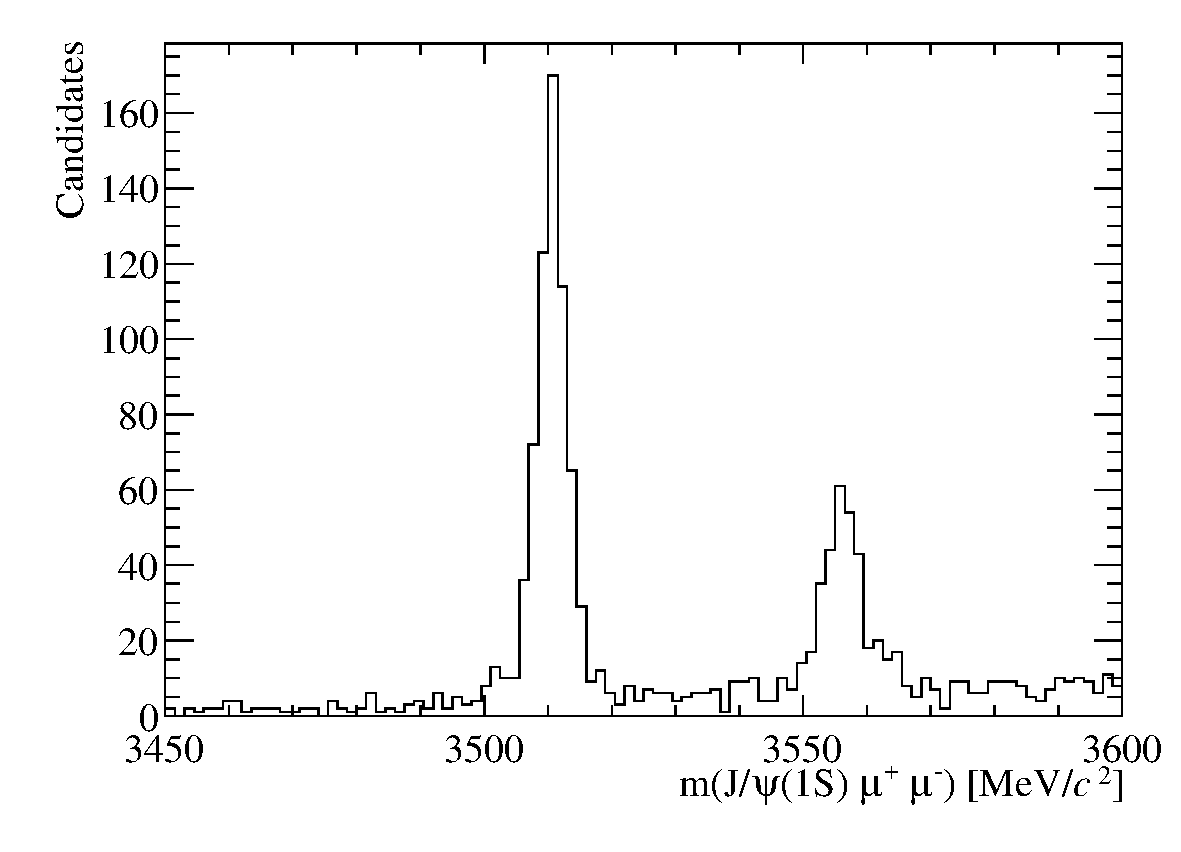
\includegraphics[width=0.75\textwidth]{figs/jmm.pdf}\\
%\caption
{\small $J/\psi \mu^+ \mu^-$ invariant mass distribution.}
%\label{fig:dmass}
\end{center}
%\end{figure}
%

Download the files chic.bin and jmm.bin files  from the DAH Dropbox, 
These files contain the data recorded by LHCb during Run 1. Focus on the chic.bin file, which selects only the invariant mass distribution around the $\chi_{c1}$ and $\chi_{c2}$ peaks. 
The files are written in binary format and contain six observables
\begin{itemize}
\item  invariant mass of $J/\psi \mu^+ \mu^-$  candidate  in  MeV/$c^2$;
\item  invariant mass of the muon pair from the virtual photon   MeV/$c^2$;
\item transverse momentum of  $J/\psi \mu^+ \mu^-$   candidate  MeV/$c$;
\item Minimum transverse momentum of the two muons in MeV/$c$;
\item Minimum of a variable (ProbNNmu) that characterizes how well the two tracks forming the candidate match the hypothesis of being muons;
\item Minimum impact parameter $\chi^2$ of the two muons. The impact parameter characterizes how well the particle is matched as coming directly from a proton-proton interaction. For tracks from
 $b-$decays it should be large.
\end{itemize}

Write a python script that reads the data from this file, see below. 
\lstinputlisting{../scripts/project_F_d.py}
%\vspace*{-0.5cm}

\begin{enumerate}

\item Plot histograms of all six variables, choosing a reasonable bin width. Always label plots correctly with title and axes and save these to a file. [Hint: The bin width should be chosen such that each of the three peaks is clearly resolved and represented by a sufficient number of bins for analysis.]

\item Next, make some estimates of the peak positions and widths using the histogram of invariant mass.  Determine the masses of the two particles by determining the bins with the highest number of entries in the peak regions. Divide the histogram into two peak regions and write a local peak finding method for this part. What is the mass differences between the $\chi_{c2}$ and $\chi_{c1}$ states ? By inspecting visually the muon-pair mass spectrum, determine the Full Width Half Maximum (FWHM) of the $\chi_{c2}$ and $\chi_{c1}$ mass peaks. Assuming a Gaussian signal shape estimate the mass resolution $\sigma$ from the FWHMs. Look up the properties of the $\chi_{c1}$ and $\chi_{c2}$ in the PDG and comment on the origin of the peak width for the two resonances.

\item In the  mass spectrum define a signal region of width $\pm 8\; {\rm MeV}/c^2$ around the $\chi_{c1}$  peak position and determine the number of events $N$ in this region. Define an upper and lower sideband region where there are only background events. These sidebands should each be half as wide as the signal region and located at masses equidistant from the $\chi_{c1}$  peak position. Assuming that the background is falling linearly with the muon-pair mass, determine the number of background events $B$ in the signal region (below the $\chi_{c1}$ peak). Perform either a linear least squares fit in the sideband regions or use the sideband subtraction method for this. Determine the number of signal events $S$ in the signal region.

\item Consider first the $\chi_{c1}$ peak which is the particle with the lowest
mass, i.e. the left most peak in the plot. Construct a composite probability density
function (PDF) for the invariant mass of the muon pairs, which
contains two components : 
\begin{itemize}
\item A Gaussian shape to fit the  $\chi_{c1}$ mass peak;
\item A shallow falling exponential to fit the background shape of the mass spectrum underneath and around the peak.
\end{itemize}

\item	Use this PDF in a Maximum Likelihood fit to determine the parameters of the PDF. Note hat it is essential that the composite PDF remains normalised to 1 over the range of the fit.

Determine the $\chi_{c1}$  meson mass and yield, and all other parameters, and their and errors.

You should be able to obtain the parameter errors directly from the minimization engine of your choice (scipy.optimize.minimise, scipy.optimise.curve\_fit, lmfit, see \url{https://lmfit.github.io/lmfit-py/} or Minuit). Depending on your choice you will be able to chose different minimising methods.
It would be good to show that you understand these by obtaining them yourself from the parameters of the Gaussian signal fit - this is described in the data handling lectures.

Plot the fitted signal shape on top of the data.

\item Now consider the entire mass range, and perform a simultaneous fit for both
peaks, and the underlying background. Again you should always report the parameter
values, and their errors. Plot the fitted signal shape on top of the data.
\item The results so far probably look quite good by eye. i.e. the signal shape plotted on
top of the data probably looks like it fits quite well. However this can be misleading
when performing a precision measurement. You should make a plot of what are called
the residuals. A residual is the difference between the data in the binned histogram
and the best-fit mass model value for the centre of that bin. Describe what you see.
\item There are several ways to enhance the scope of the project.

\begin{itemize}
\item The second file (jmm.bin) extends the $J/\psi \mu^+ \mu^-$ mass range to higher values. At higher masses more states are expected - for example radial excitations of the $\chi_c$ together with more exotic things. Plot the invariant mass distribution and with the help of the PDG try to identify the peaks you see. The other variables in the file can be used to help improve the purity of the sample and make peaks clearer. Try to fit some of the additional peaks and determine the yield and position.
\item Going to higher masses allows the production of vector mesons such as the $\phi(1020)$. This state can decay to a dimuon pair. Try selecting candidates within $\pm 10\; {\rm MeV}/c^2$ of the $\phi$ mass using the second column in the datafile. Plot the $J/\psi \mu+ \mu^-$  invariant mass distribution and with the help of the PDG try to identify the peaks you see. Again try to fit the peaks.
\item Consider replacing the Gaussian with a Voigt function. The functional shape is described elsewhere, e.g. see:
\begin{verbatim}
https://en.wikipedia.org/wiki/Voigt_profile 
\end{verbatim} 
You could implement this function in your PDF (with some help from scipy) and try to separate the contributions from the natural width and detector resolution to the line shape. Try to understand why the voigt is a better physical description of the data.

\end{itemize}



\end{enumerate}

\subsection{Project planning}

The project descriptions are generally significantly less detailed than what was made available for the checkpoints. Any material covered during checkpoints including python code examples are assumed to be known.  Only essential and new information is provided and you are expected to take care of the details. Python code snippets are provided where necessary, but you will have to understand yourself what they do. It is recommend that you google for information about your project on the web, including data sheets of components and python libraries, if applicable. Python scripts should be well structured, either using functions or classes.

The timeline will vary between different projects, but in general, it is recommended that you plan your work as follows:
\begin{itemize}
\item	weeks 7, 8 \& 9: 	Building your gadget and/or writing code for project;
\item	week 9, 10: 	Analysis of data or equivalent, prepare supplementary material;
\item	week 10, 11:	Finish writing of project report and prepare submission.
\end{itemize}
Note that you are advised to start writing your report as the project progresses. 

For guidance on report writing, how the projects will be assessed, plagiarism and the submission deadline, please consult the DAH course booklet and the DAH grade descriptors, available on Learn.

 


\newpage
\section{Project F5: Studies of $B^+ \rightarrow J/\psi K^+$}
%
You will use LHCb data to study the decay  $B^+ \rightarrow J/\psi K^+$. You will first make simple checks of the data and get first estimates of mass peak position and width. You will use the maximum likelihood process to fit different mass model shapes to the data. From this you will determine the parameters of the mass model for the signal peaks, and their errors. You will start with a very simple Gaussian mass model. You will then improve this and use a more sophisticated model. 

The projects have an open-ended aspect and are an opportunity where you can show your own initiative and demonstrate your experimental and computational skills.




\subsection{Detailed project description}
%
Large samples of the decay $B^+ \rightarrow J/\psi K^+$ have been collected by LHCb during its running. A very clean signal for this decay is observed and can be used to study a wealth of physics: $b$-hadron production, the $B^+$ lifetime and CP violation.The figure below shows the invariant mass distribution of selected candidates.
For more information see: {DOI:10.1007/JHEP12(2017)026}. 
%
%\begin{figure}[htb!]
\begin{center}
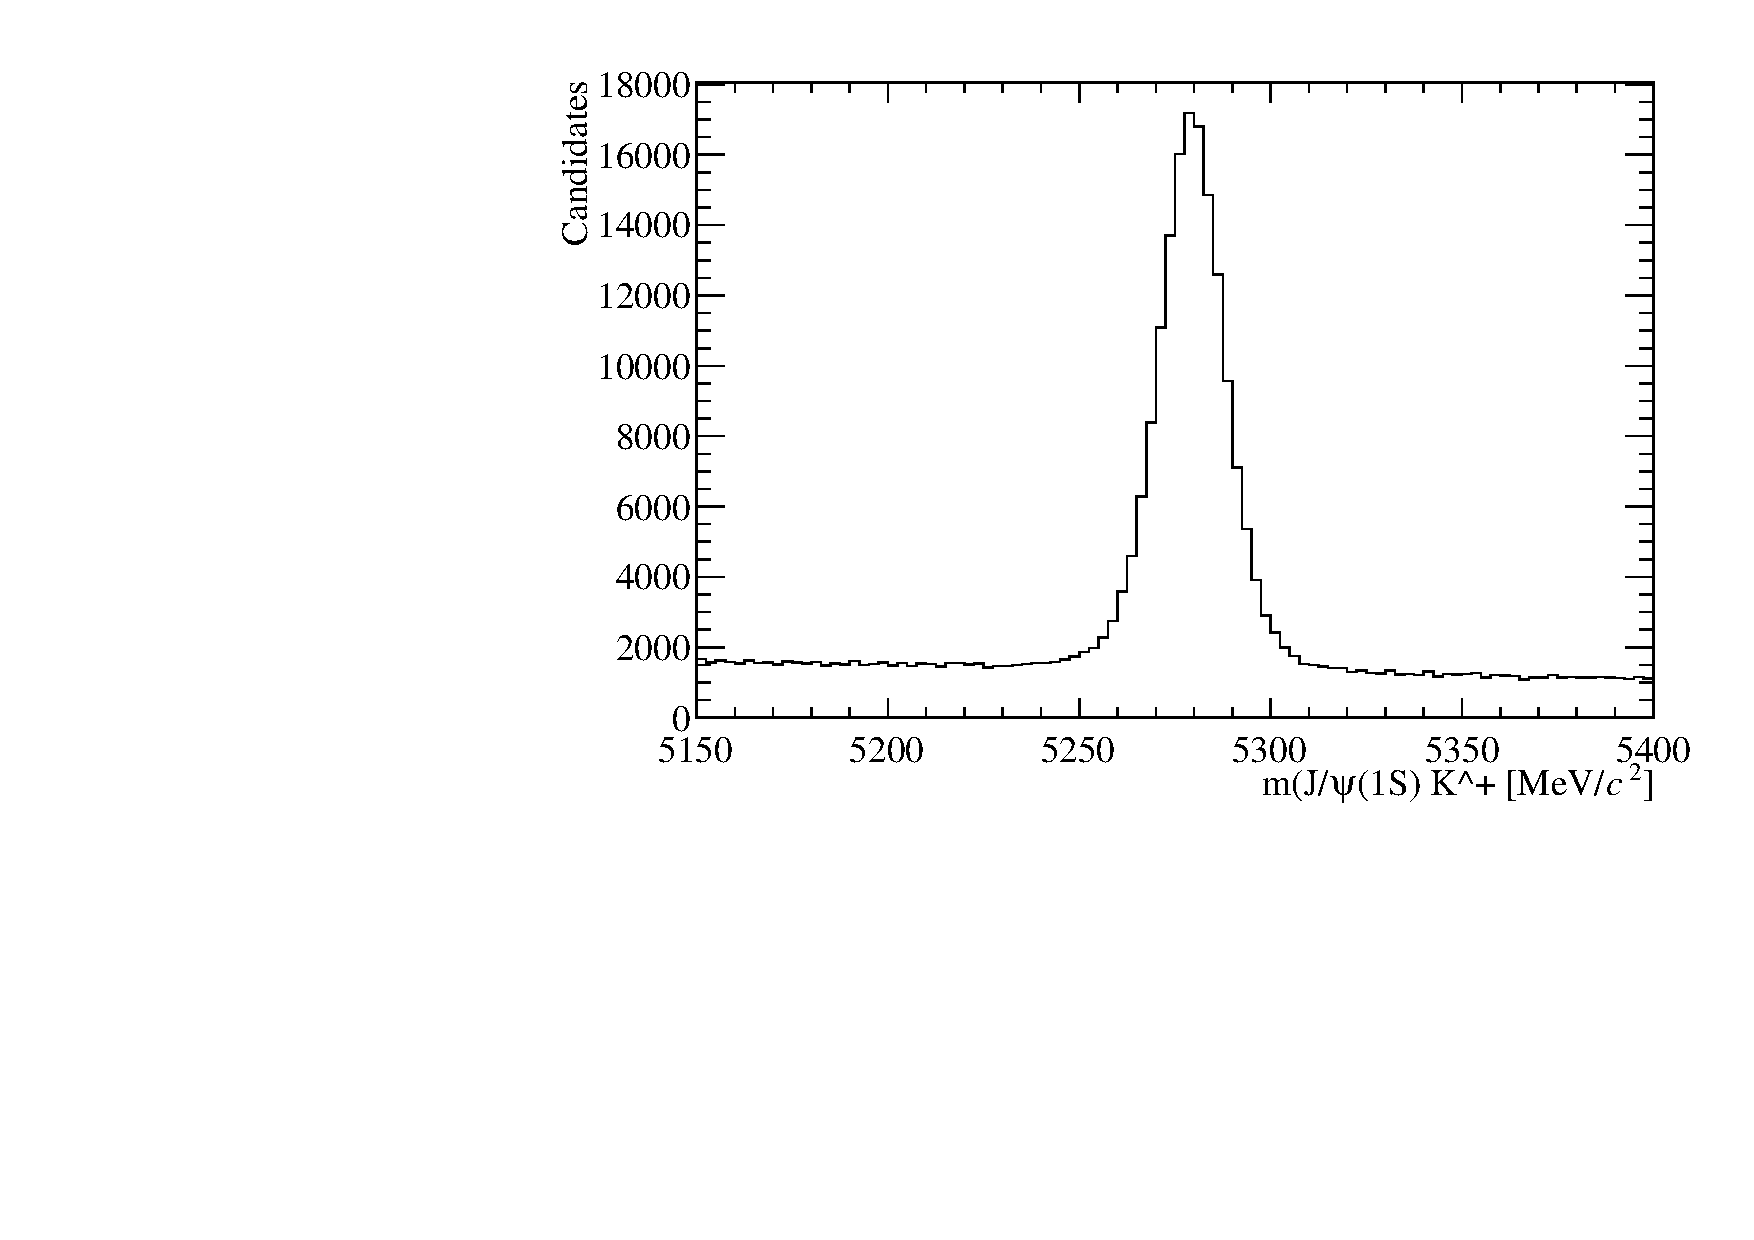
\includegraphics[width=0.75\textwidth]{figs/bmass.pdf}\\
%\caption
{\small $J/\psi K^+$ invariant mass distribution.}
%\label{fig:dmass}
\end{center}
%\end{figure}
%

Download the files kdata-small.bin and kdata.bin files  from the DAH Dropbox, 
These files contain the data recorded by LHCb during Run 1. Focus on the kdata-small.bin file,  at first which contains only a fraction of the events. 
The files are written in binary format and contain five observables
\begin{itemize}
\item  invariant mass of $J/\psi K^+$  candidate  in  MeV/$c^2$;
\item transverse momentum of  $J/\psi K^+$   candidate  MeV/$c$;
\item pseudorapidity of  $J/\psi K^+$   candidate  MeV/$c$;
\item Charge of the  candidate
\item Lifetime of the candidate in $ps$
\end{itemize}

Write a python script that reads the data from this file, see below. 
\lstinputlisting{../scripts/project_F_e.py}
%\vspace*{-0.5cm}

\begin{enumerate}

\item Plot histograms of all five variables, choosing a reasonable bin width. Always label plots correctly with title and axes and save these to a file. [Hint: The bin width should be chosen such that each of the three peaks is clearly resolved and represented by a sufficient number of bins for analysis.]

\item Next, make some estimates of the peak positions and widths using the histogram of invariant mass.  Determine the mass of the $B^+$  by determining the bins with the highest number of entries in the peak regions. Write a local peak finding method for this part. By inspecting visually the mass spectrum, determine the Full Width Half Maximum (FWHM) of the mass peak. Assuming a Gaussian signal shape estimate the mass resolution $\sigma$ from the FWHMs. How does you result for the mass compare to the PDG.

\item In the  mass spectrum define a signal region of width $\pm 25\; {\rm MeV}/c^2$ around the $B^+$  peak position and determine the number of events $N$ in this region.
  Define an upper and lower sideband region where there are only background events. These sidebands should each be half as wide as the signal region and located at masses equidistant from the peak position. Assuming that the background is falling linearly with the muon-pair mass, determine the number of background events $B$ in the signal region. Perform either a linear least squares fit in the sideband regions or use the sideband subtraction method for this. Determine the number of signal events $S$ in the signal region.

\item Construct a composite probability density
function (PDF) for the invariant mass of the muon pairs, which
contains two components : 
\begin{itemize}
\item A Gaussian shape to fit the  $B^+$ mass peak;
\item A shallow falling exponential to fit the background shape of the mass spectrum underneath and around the peak.
\end{itemize}

\item	Use this PDF in a Maximum Likelihood fit to determine the parameters of the PDF. Note hat it is essential that the composite PDF remains normalised to 1 over the range of the fit. Determine the $B^+$ meson mass and yield, and all other parameters, and their and errors.

You should be able to obtain the parameter errors directly from the minimization engine of your choice (scipy.optimize.minimise, scipy.optimise.curve\_fit, lmfit, see \url{https://lmfit.github.io/lmfit-py/} or Minuit). Depending on your choice you will be able to chose different minimising methods.
It would be good to show that you understand these by obtaining them yourself from the parameters of the Gaussian signal fit - this is described in the data handling lectures.

Plot the fitted signal shape on top of the data.

\item Now consider the entire mass range, and perform a simultaneous fit for both
peaks, and the underlying background. Again you should always report the parameter
values, and their errors. Plot the fitted signal shape on top of the data.
\item The results so far probably look quite good by eye. i.e. the signal shape plotted on
top of the data probably looks like it fits quite well. However this can be misleading
when performing a precision measurement. You should make a plot of what are called
the residuals. A residual is the difference between the data in the binned histogram
and the best-fit mass model value for the centre of that bin. Describe what you see.
\item Divide the data into $B^+$ and $B^-$ and repeat the exercise.

\item There are several ways to enhance the scope of the project. For theses studies consider to use the bigger file (kdata.bin)
  \begin{itemize}
\item If the single Gaussian mass model does not fit the data perfectly, one can try other mass models, i.e. by using a signal PDF that goes beyond a single Gaussian function.  Examples are:
\begin{itemize}
\item A PDF comprising a function which is the sum of two Gaussian functions (i.e. one narrow and one wide Gaussian function to fit the mass peak)
\item A Crystal Ball function, which incorporates a non-Gaussian tail at the lower end of the mass peak. The functional shape is described elsewhere, e.g. see: \url{http://en.wikipedia.org/wiki/Crystal_Ball_function}. 
\end{itemize}
Implement one or both of these functions in your PDF.
\item Fit the data in bins of lifetime and plot the yield in bins of time. Try to extract the lifetime of the $B^+$.
\item Perform the fit in bins of $pt$ and pseudorapidity. Compare the results to the studies of $B^+$ production in the paper and the predictions available online at
\begin{verbatim}
  http://www.lpthe.jussieu.fr/~cacciari/fonll/fonllform.html 
\end{verbatim} 

\end{itemize}
\end{enumerate}

\subsection{Project planning}

The project descriptions are generally significantly less detailed than what was made available for the checkpoints. Any material covered during checkpoints including python code examples are assumed to be known.  Only essential and new information is provided and you are expected to take care of the details. Python code snippets are provided where necessary, but you will have to understand yourself what they do. It is recommend that you google for information about your project on the web, including data sheets of components and python libraries, if applicable. Python scripts should be well structured, either using functions or classes.

The timeline will vary between different projects, but in general, it is recommended that you plan your work as follows:
\begin{itemize}
\item	weeks 7, 8 \& 9: 	Building your gadget and/or writing code for project;
\item	week 9, 10: 	Analysis of data or equivalent, prepare supplementary material;
\item	week 10, 11:	Finish writing of project report and prepare submission.
\end{itemize}
Note that you are advised to start writing your report as the project progresses. 

For guidance on report writing, how the projects will be assessed, plagiarism and the submission deadline, please consult the DAH course booklet and the DAH grade descriptors, available on Learn.

 




\begin{comment}
\newpage
\section{Project F3old: Make Accurate Measurements of Particle Masses}

\subsection{Goals of project}

You will use LHCb data on the invariant mass of particle candidates that you were introduced to during a checkpoint. You will analyse this in a much more sophisticated way and closer to the actual analysis performed leading to its publication. You will use the maximum likelihood process to fit different mass model shapes to the data. From this you will determine the parameters of the mass model for the three signal peaks, and their errors. You will start with a very simple Gaussian mass model. You will then improve this and use a more sophisticated model.

The projects have an open-ended aspect and are an opportunity where you can show your own initiative and demonstrate your experimental and computational skills. 



\subsection{Detailed project description}

You were previously introduced to the LHCb Upsilon data. In this
project you will explore another LHCb dataset where a $\psi(2S)$ meson
(a bound $c\overline{c}$ state) and a pair of
oppositely pions have been combined. Two clear
peaks are observed in this mass spectrum corresponding to the $B_s$
and $B^0$ mesons, see figure below %(Fig.~\ref{fig:bmass}). 
The background shape is quite
complex. At higher masses it is exponential in shape. At lower masses
there is an additional background from the decay $B^0 \rightarrow
\psi(2S) K^+ \pi^-$ where the kaon has been incorrectly identified as
a pion. For more information see: {DOI: 10.1016/j.nuclphysb.2013.03.004 and DOI: 10.1016/j.physletb.2015.06.038}.


During checkpoint 6, you performed some very simple "peak finding". In this project you are going to do the analysis much like it would actually be carried out in a particle physics experiment.

%
%\begin{figure}[htb!]
\begin{center}
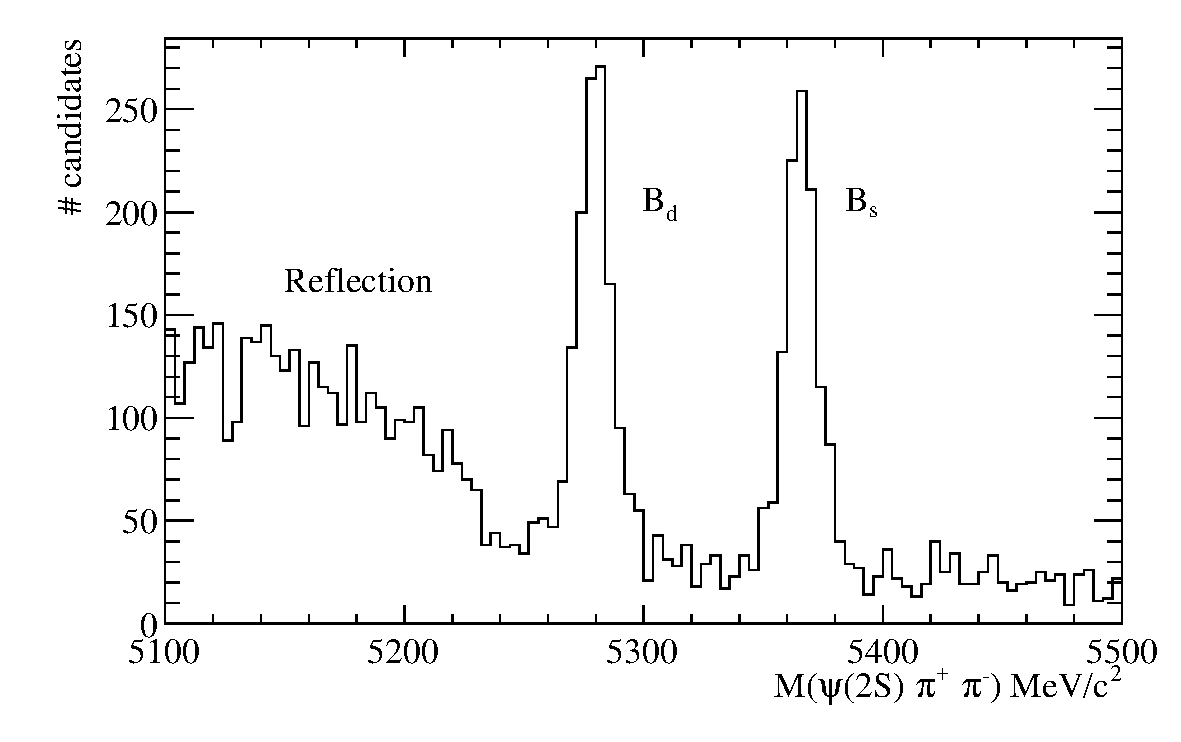
\includegraphics[width=0.75\textwidth]{figs/psi2Spipi.pdf}\\
%\caption
{\small $\psi ({\rm 2S}) \pi^{+} \pi^{-}$  invariant mass distribution.}
%\label{fig:bmass}
\end{center}
%\end{figure}
%


\begin{enumerate}


\item Consider first the $B_s$ peak which is the particle with the highest
mass, i.e. the right most peak in the plot. Construct a composite probability density
function (PDF) for the invariant mass of the muon pairs, which
contains two components :

\begin{itemize}
\item A Gaussian shape to fit the $B_s$ peak;
\item A shallow falling exponential to fit the background shape of the mass spectrum
underneath the peak.
\end{itemize}

\item Use this PDF in a Maximum Likelihood fit to determine the parameters of the PDF.
Note hat it is essential that the composite PDF remains normalised to 1 over the range
of the fit. 

Determine the $B_s$ meson mass and yield, and all other parameters, and their and
errors.

You should be able to obtain the parameter errors directly from the minimization engine of your choice (scipy.optimize.minimise, scipy.optimise.curve\_fit, lmfit, see \url{https://lmfit.github.io/lmfit-py/} or Minuit). Depending on your choice you will be able to chose different minimising methods.
It would be good to show that you understand these by obtaining them yourself from the parameters of the Gaussian signal fit - this is described in the data handling lectures.

Plot the fitted signal shape on top of the data.

\item Now consider the mass range above the reflection, and perform a simultaneous fit for both
peaks, and the underlying background. Again you should always report the parameter
values, and their errors. Plot the fitted signal shape on top of the data.

\item The results so far probably look "quite good" by eye.  i.e. the signal shape plotted on top of the data probably looks like it fits quite well.  However this can be misleading when performing a precision measurement.  You should make a plot of what are called the "residuals". A residual is the difference between the data in the binned histogram and the best-fit mass model value for the centre of that bin. Describe what you see.

\newpage

\item There are several ways to enhance the scope of the project.

\begin{itemize} 
\item For example, if the single
Gaussian mass model does not fit the data perfectly, one can try other mass models,
i.e. by using a signal PDF that goes beyond a single Gaussian
function. One example: is a PDF comprising a function which is the sum of two Gaussian functions (i.e. one
narrow and one wide Gaussian function to fit a single D meson
peak. Alternatively try a Crystal Ball function, which incorporates a non-Gaussian tail at the lower end of
the mass peak. The functional shape is described elsewhere, e.g. see:
\begin{verbatim}
https://en.wikipedia.org/wiki/Crystal_Ball_function 
\end{verbatim} 
You could implement each of these functions in your PDF and see how much better
they are at describing the data.
\item Try to extend the fit to include the kinematic reflection
\item Read the publication and see what is said about systematic errors. Make a reasonable
attempt at determining some systematic errors on the masses.
\item Compare your results to the PDG and previous measurements.
\item From the yields of $B_s$ and $B^0$ mesons, following the
  procedures in the papers try to evaluate the ratio of branching
  ratios of these modes.
\end{itemize}


\end{enumerate}

\subsection{Project planning}

The project descriptions are generally significantly less detailed than what was made available for the checkpoints. Any material covered during checkpoints including python code examples are assumed to be known.  Only essential and new information is provided and you are expected to take care of the details. Python code snippets are provided where necessary, but you will have to understand yourself what they do. It is recommend that you google for information about your project on the web, including data sheets of components and python libraries, if applicable. Python scripts should be well structured, either using functions or classes.

The timeline will vary between different projects, but in general, it is recommended that you plan your work as follows:
\begin{itemize}
\item	weeks 7, 8 \& 9: 	Building your gadget and/or writing code for project;
\item	week 9, 10: 	Analysis of data or equivalent, prepare supplementary material;
\item	week 10, 11:	Finish writing of project report and prepare submission.
\end{itemize}
Note that you are advised to start writing your report as the project progresses. 

For guidance on report writing, how the projects will be assessed, plagiarism and the submission deadline, please consult the DAH course booklet and the DAH grade descriptors, available on Learn.

 
\end{comment}



%\chapter{DAH: Remote connection guide}
\label{sec:remote}

All of these techniques are tested as best we can, but rely on external software that may have its own problems.
If you have issues, please contact b.m.wynne@ed.ac.uk

\section{SSH connection to Raspberry Pi}

All Raspberry Pis in the DAH labs should be accessible via an SSH connection, assuming they are switched on.
To access one, first log into the Student Gateway machine:
\begin{verbatim}
  ssh -Y yourUUN@student.ph.ed.ac.uk
\end{verbatim}

Once you have logged into the Student Gateway (using your regular university username and password) you can now access the DAH labs.
\begin{verbatim}
  ssh -Y studentAA@dahpiBB
\end{verbatim}

For AA and BB you should substitute the student number you were given to login in the lab, and the number of the Pi that you were using.
Your login will work on any of the Pis, but please use the one you have been assigned unless it is not available.

Once you have access to the Pi, you should be able to retrieve or run any code that you have written.
If you are not familiar with the Linux command line, try using the ``nano'' editor to view or change files.

To download files from the Pi, it might be helpful to use FTP.
Log into the Student Gateway computer like before, but now connect to the Pi like this:
\begin{verbatim}
  sftp studentAA@dahpiBB
\end{verbatim}

You are now in a limited command-line environment that will respond to instructions like ``ls'' and ``cd'' to navigate the filesystem.
To download (for example) the file ``myTestFile.txt'' you would run the following command:
\begin{verbatim}
  get myTestFile.txt
\end{verbatim}

This file will now be available in your standard university account.
To close the connection to the Pi, or to the Student Gateway, simply type ``exit'' --- typing this while logged into the Pi will return you to the Student Gateway.


\section{Using a graphical interface remotely}

We do not support the option for you to run the full Pi desktop environment remotely.
However, you will be able to run programs with a GUI from the command line, and then see the GUI on your own machine.

If your own computer is running a Linux-based operating system then this will happen automatically, if you follow the instructions above.
You can test this by attempting to open a GUI-based program, such as ``geany'' the Python code editor.

If your computer is running Mac OS or Windows, you may need additional software, as described below.

\subsection{Windows}

(This information is based on \href{https://superuser.com/questions/119792/how-to-use-x11-forwarding-with-putty}{this webpage})

Viewing GUI programs from the Raspberry Pi in Windows will require you to have an SSH client that supports X-window forwarding, and an X-window server.
There are several options, but I strongly recommend using \href{https://www.putty.org/}{PuTTY} and \href{https://sourceforge.net/projects/vcxsrv/}{vcxsrv} as the client and server respectively.

Install both programs, and ensure that vcxsrv is running.
Now open PuTTY and configure it to allow X-window forwarding as shown:
\begin{center}
  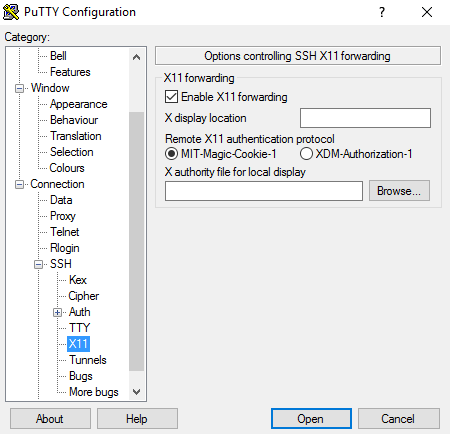
\includegraphics[width=14cm]{figs/PuttyXwin}
\end{center}

Use PuTTY to connect to the Student Gateway, and then follow the original instructions from that point.

\subsection{MacOS}

(This information is based on \href{https://www.youtube.com/watch?v=s6e3cqCISaE}{this video})

Viewing GUI programs from the Raspberry Pi in MacOS X will require you to install the \href{https://www.xquartz.org/}{XQuartz} application.
Once it is installed, start it running and open the Applications menu (you will not see anything other than the XQuartz menu bar at this point).
Select Terminal to create a new command line interface.
You can now follow the original instructions, connecting to the Student Gateway from within this terminal window.


%\chapter{DAH Quiz}
\label{sec:quiz}

Solve the following questions about data acquisition and handling material on your own time,
i.e. you should not use the laboratory hours to solve the quiz questions. 
In total, 20 marks can be obtained.
The quiz will count for 10\% of the total course mark, see also the course booklet. 

Please hand in your solutions to the questions to the Teaching Office.

{\bf Deadline:} 12 noon, Tuesday, 6$^{th}$ November 2018.

\begin{enumerate}

\item  In a particle physics experiment at the Large Hadron Collider at CERN, photons  are recorded in an electromagnetic crystal calorimeter. Each crystal is read out with a photodetector and the signals
are  digitised with an Analog-to-Digital Converter (ADC).
%
\begin{itemize}
%\item With the aid of a diagram, explain briefly how an ADC works.
\item In order to measure photon  energies  in  the dynamic range of 40 MeV to  2.0 TeV,
how many bits are required for the ADC? 
%\item In practise, the energy deposited in a crystal is measured with multiple 12-bit ADC channels %which cover low and high energy ranges separately by using  a multi gain preamplifer, see figure.
%Show that the gain factors 1, 6 and 12 are sufficient to cover the full dynamic range.
\end{itemize}
[ Hint: 1 TeV = $10^{12}\; \rm eV$, 1 GeV = $10^9\; \rm eV$ and 1 MeV = $10^6\; \rm eV\; .$ ]
%
\hfill {\bf [2 marks]}\\

%\begin{comment}
\item In DAH checkpoint (4) a PCF8574AN expander I/O chip was used to control a LED light pattern.  You were instructed to connect all address lines (A0, A1, A2) to ground which corresponds to the slave address {\tt 0x38}. What would the slave address be  if all address lines were connected to 3.3V?
Explain hexadecimal numbers. 

The I2C bus allows to connect multiple slave devices. How many PCF8574AN chips can be controlled in total from one Raspberry-Pi?

[ Hint: You need to consult the PCF8574AN data sheet. 
Note that the prefix {\tt 0x} is used for representing numbers in hexadecimal notation.  ] 
%
\hfill {\bf [2 marks]}\\
%\end{comment}

\item Charged particles traversing a drift chamber, ionise the gas and the electrons drift toward anode wires where these are multiplied in a high electric field. Thus a fast charge signal is produced which can be converted into a voltage pulse by means of a pre-amplifier. 
The drift time is a measure of the distance from where the the drift electrons were created to the anode wire.

In a particle physics experiment, a drift chamber with 384~anode wires is used to measure trajectories of charged particles. 
The drift velocity is $1\; {\rm cm/\mu s}$, the maximum drift time is $6.5 \; \mu$s
and  a spatial resolution of  better than $200\; \mu$m is needed.
What electronics equipment is required to read out the signal pulses of the drift chamber? State its main specifications.
\hfill {\bf [5 marks]}\\

\item The $^{22}$Na nuclei decays with a half-life of 2.6 years by positron emission. The positron annihilates with an electron giving rise to a pair of $\gamma$-rays with energies of 0.51 MeV. 
Coincidence measurements can be used to demonstrate that two 0.51 MeV $\gamma$-rays are produced  with the two photons travelling in opposite directions. A schematic  of the apparatus you might use to record the pairs of photons is shown below:
%
\begin{center}
 {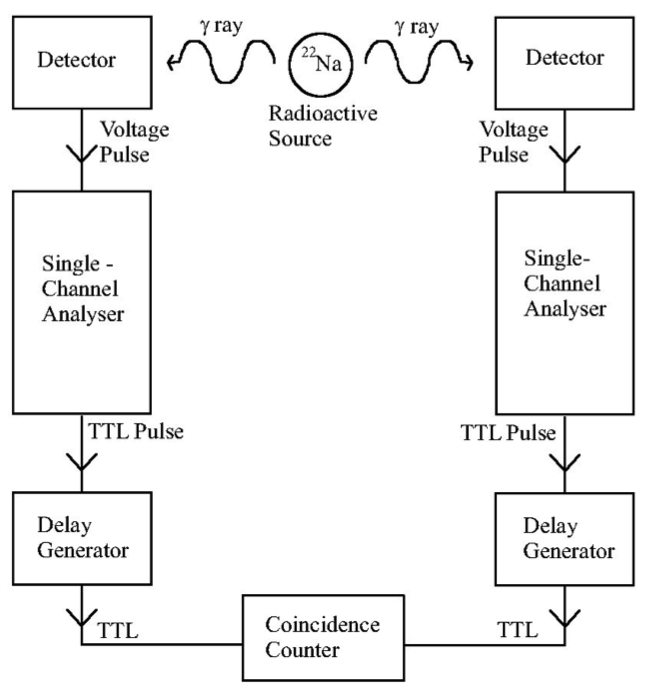
\includegraphics[width=0.35\textwidth]{figs/positron-annihilation}}
 \end{center}
%
The pulses from the detector have a peak voltage that is proportional to the energy of the $\gamma$-rays. By means of  a  single-channel analyser  a TTL pulse is  produced whenever the amplitude of the input pulse lies within a specified voltage range.
\begin{itemize}
\item With the aid of a diagram show the sequence of pulses from the detector to the coincidence unit, illustrating how a single-channel analyser works.  What does TTL stand for?
What does this imply about the output pulses of the single-channel analyser?
\item Delay generators can be used to delay the time at which one of the pulses reaches the coincidence counter.
Explain why this might be necessary. % to delay one of the pulses.
%
%\item 
%To determine whether two pulses are coincident, what logic operation is required?
\hfill {\bf [4 marks]}
%
\end{itemize}



\item A peak  in a data distribution, which is clearly visible (by eye) can usually be assigned to a signal (e.g. a particle mass, an atomic transition wavelength, ...). 

Explain what  the  resolution ($\sigma$) and the Full Width Half Maximum (FWHM)  of a signal peak in a distribution are. 
Derive the relation, FWHM$  = 2 \sqrt{2 \log 2}\; \sigma$, for the resolution $\sigma$ of a Gaussian distribution.  
\hfill {\bf [3 marks]}\\

Write a python script which uses random numbers to generate a Gaussian distribution with a mean $\mu$ and a resolution $\sigma$.
Plot a histogram of  this distribution.
Calculate the mean and variance  of the generated distribution and show 
that the results agree with your input values.
You need to submit a printout of your code and its outputs.

%[ Hint: For random numbers, use the python notes, available on Learn. ]
\hfill {\bf [4 marks]}



\begin{comment}
\item Write a short python script which generates a flat distribution and plots a histogram of  
the distribution.
Calculate the mean and variance  of the generated distribution and show that for a flat distribution between $a$ and $b$, the relation
 $\sigma = \frac{b-a}{\sqrt{12}}$  for the resolution $\sigma$ 
is satisfied. You need to submit a printout of your code.

Derive the  relation $\sigma = \frac{b-a}{\sqrt{12}}$ for the resolution $\sigma$ of a flat distribution between $a$ and $b$.  

\hfill {\bf [6 marks]}
\end{comment}

\end{enumerate} 





\end{document}
